\section{Empirical Results}
\label{CH:EmpiricalResults}


For the empirical application of the proposed model, we investigate the evolution of the IBM stock price. The data comes from the TAQ database of the New York Stock Exchange in the period from January 2nd, 2001 to December 30th, 2018. The price is sampled in intervals of $5$ minutes and contains $4444$ trading days, excluding holidays and weekends. The time series for our application will be the daily realized volatility introduced in section \ref{CH:Application:RV}. In order to compare the models that come from the Reservoir Computing field with the HAR model by \cite{Corsi2009}, we take the log transformation of the daily realized volatility. So our time series becomes
\begin{eqnarray}
    u_t = \log{\sqrt{RVD_t}} = \log{\sqrt{\sum_{j=1}^{78} r_{t_j}^2}}
\end{eqnarray}
where $r_{t_j}$ is referring to the $j$-th $5$-minute return on day $t$. The core trading hours on the New York Stock Exchange are from 9:30 am to 4:00 pm\footnote{https://www.nyse.com/markets/hours-calendars}, which amounts to $6.5$ hours or $87$ intervals of $5$ minutes.

Figure \ref{FIG:IBMRVAR:Series} presents the evolution of the realized volatility of IBM in the given timeframe. The left panel is referring to the original series of $\sigma_t$ and the right panel is its log transformation $\log{\sigma_t}$. 

Especially in the early years of the 21st century, the aftermath of the burtst of the 'dot com' bubble are still present in the timeseries which IBM as a technology company was probably more affected than other companies as well as the effect of the global financial crisis of 2007/2008 where this specific company was less affected by than in the early years of the century. Calmer periods of low volatility can be seen in the years between 2004 and 2006 and between late 2012 and late 2015 which underlines the presence of clustering.

Apart from the idiosyncratic risks associated to IBM, the evolution shows the typical patterns of volatility in financial time series, namely clustering and high persistence. Clustering is describing the pheonomenon of periods of high volatility being followed by periods of low volatility. High persistence is referring to a high level of autocorraltion which is presented in figure \ref{FIG:IBMRVAR:Autocorr}. The blue shaded area covers the range of significant autocorrelation and is touched for the first time at approximately the $140$-th lag. This corresponds to more than $6$ months. 


\begin{figure}
    \begin{center}
        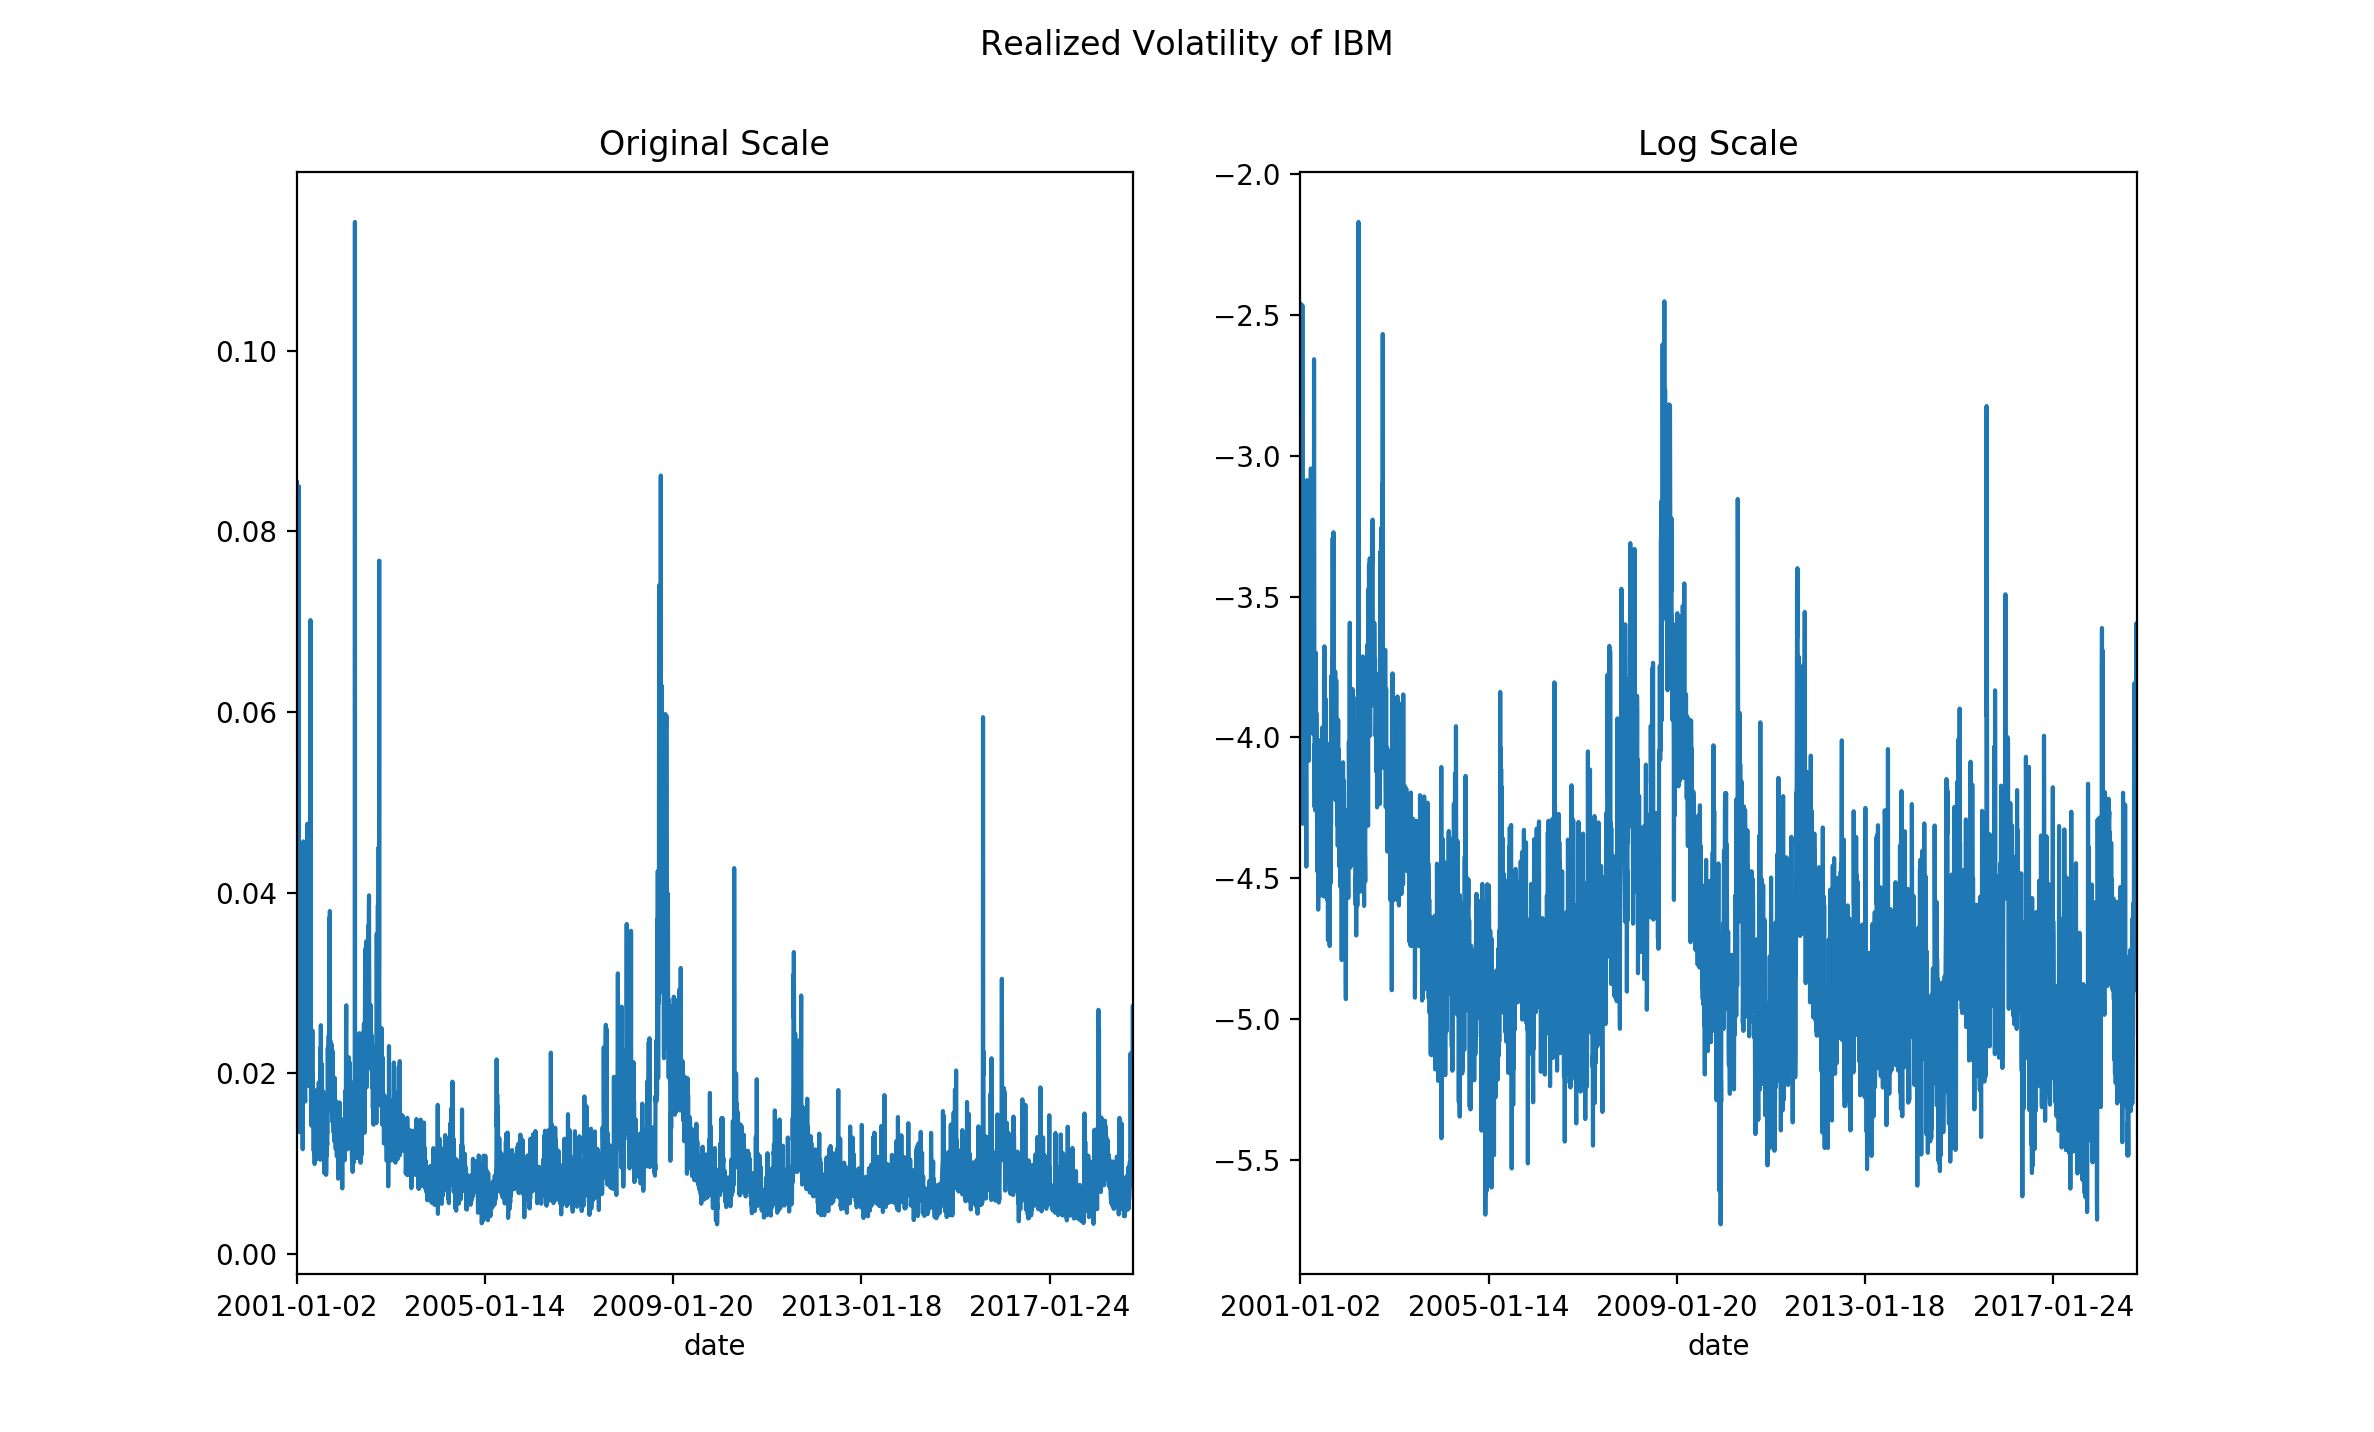
\includegraphics[width=\textwidth]{Plots/IBM_RVAR.png}
    \end{center}
    \caption{Realized volatility of IBM for the period from January 2nd, 2001 to December 30th, 2018. The left hand side presents the realized volatility in its original scale, the right hand side presents the log transformation of the time series.}
    \label{FIG:IBMRVAR:Series}
\end{figure}

\begin{figure}
    \begin{center}
        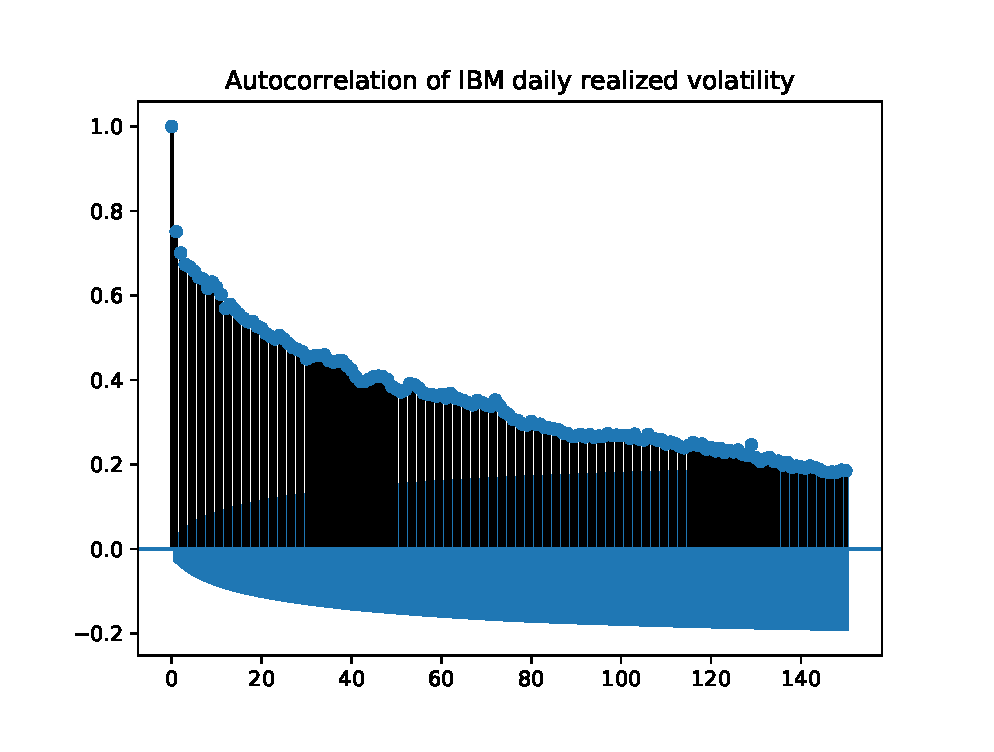
\includegraphics[width=\textwidth]{Plots/IBM_RVAR_autocorr.eps}
    \end{center}
    \caption{Autocorrelation of daily realized volatility of IBM for the period from January 2nd, 2010 to December 30th, 2018. The blue shaded area are the bounds for significance which is touched for the first time at approximately the $140$-th lag which shows the long persistence in the series.}
    \label{FIG:IBMRVAR:Autocorr}
\end{figure}

In what follows, we will refer to the loss induces experts as \textit{loss experts} and to the plasticity weighted experts as \textit{plasticity experts}.

\subsection{Analysis of Network Behaviour}

In this section we want to shed some more light of the network behaviour for reservoirs that have been pre-trained using the intrinsic plasticity approach from section \ref{CH:ESN:Tuning} using the IBM realized volatility as input $u_t$.
Figure \ref{FIG:NetworkActivations} presents the network activations for a givent time period and compares two networks that have been pre-trained towards different normal distributions. Networks of size $n=200$ were used and the network has been presented the whole time series of realized volatilities for $100$ epochs of adaptation. Given the $tanh$ activation function as well as the scaling of the input series to $[-0.8, 0.8]$ support the centering of network activations around $0$ which is in line with setting the mean $\mu = 0$ that has been argued about in section \ref{CH:ExpertModels}. The network behaviour for the left panel, which has been targeted towards $\mathcal{N}(0, 0.16)$, barely manages to put the neurons' output inside the $95\%$ confidence bounds of the respective normal distribution. In periods of relatively low volatility, e.g. between step $10$ and $20$ or around step $90$, the network is able to fit the normal distribution relatively well. This compares to the network in the right panel, where the network has been trained to match a normal distribution $\mathcal{N}(0,1)$. Here the adaptation barely manages to fit the neurons activations outside the confidence bounds\footnote{Given the size of the reservoir, approximately $0.05\cdot 200 = 10$ activations should lie outside the confidence bounds}.

% \begin{figure}
%     \begin{center}
%         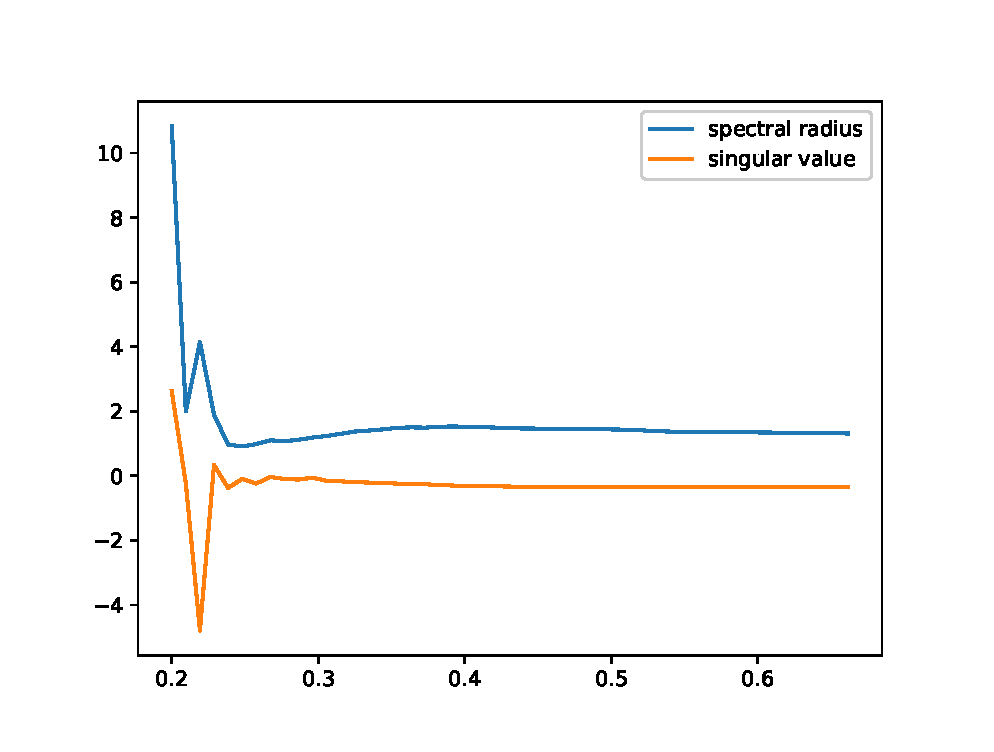
\includegraphics[width=\textwidth]{Plots/spectral_radius.eps}
%     \end{center}
%     \caption{foo}
%     \label{FIG:SpectralRadius}
% \end{figure}


\begin{figure}
    \begin{center}
        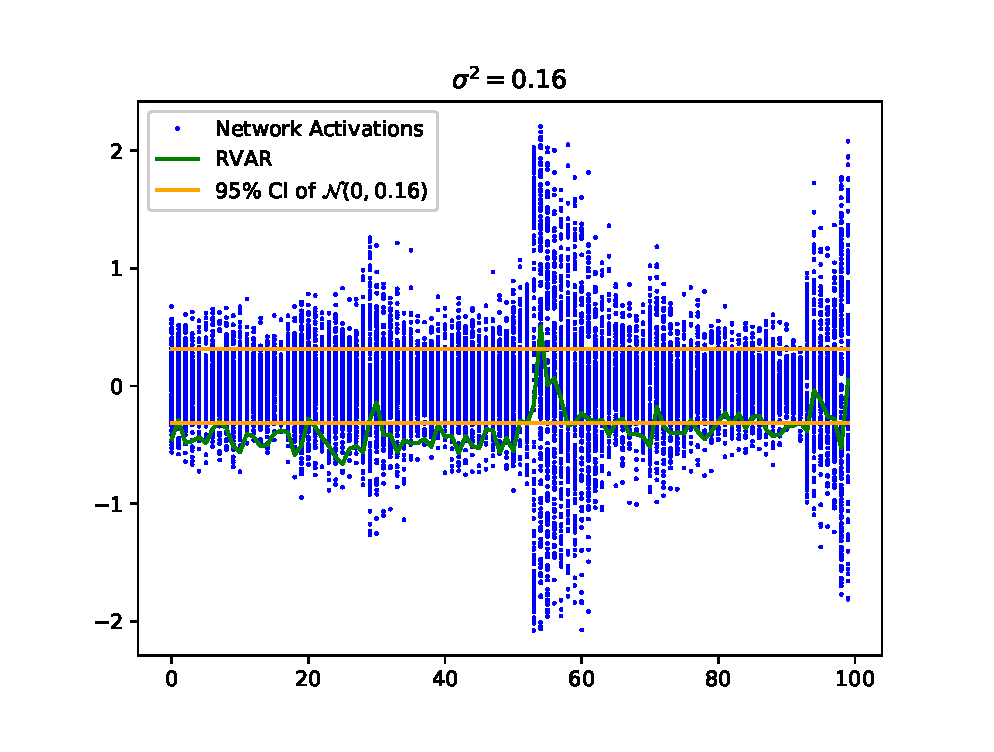
\includegraphics[width=0.49\textwidth]{Plots/network_activation_016.eps}
        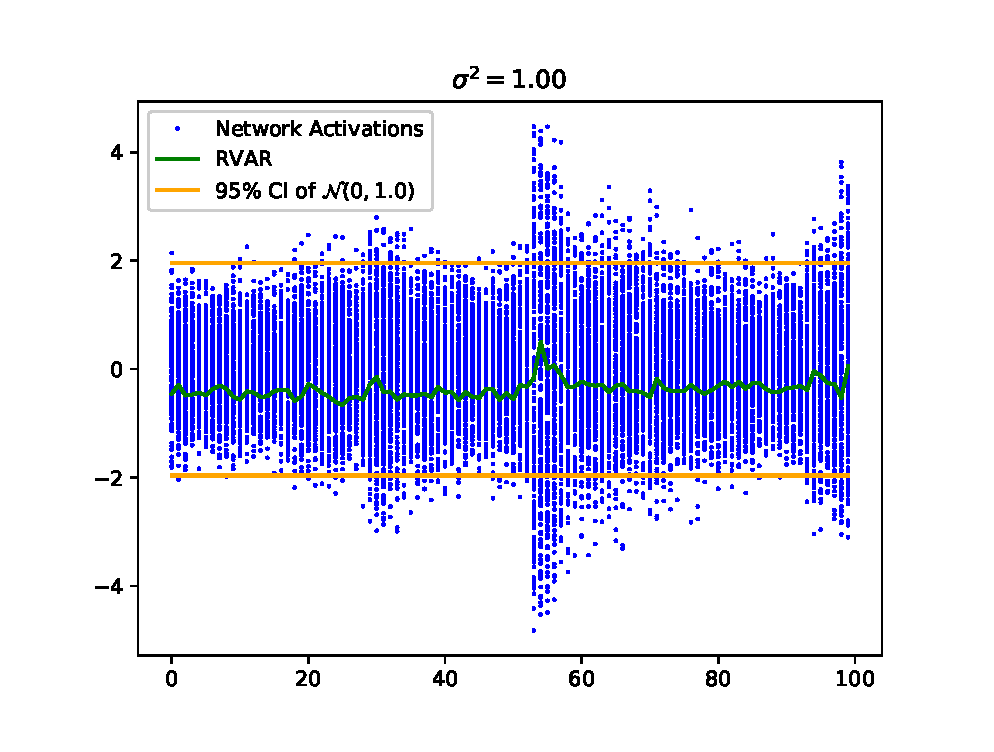
\includegraphics[width=0.49\textwidth]{Plots/network_activation_10.eps}
    \end{center}
    \caption{Comparison of the activations for two different plasticity tuned networks. One has been tuned for $\sigma = \frac{1}{\sqrt{2\pi}} = 0.16$ which we will use later in the empirical application. As a comparison, a network with $\sigma = 1.0$ is presented. The horizontal lines are the $95\%$ confidence bounds to give an idea of the range of a normal distribution $\mathcal{N}(0, \sigma^2)$ with the corresponding parameters. The time series presented is from 10th of July to 30th of October 2015. It has been rescaled to the interval $[-0.8, 0.8]$ and was chosen for representative purposes only. Comparing the two, one can see that the extreme values of the timeseries around step $55$ make the network with $\sigma = 0.16$ very unlikely given the amount of activations outside the confidence bounds. The effect of this move on the network with $\sigma = 1.0$ is much less significant when considering the comparably fewer activations outside the bounds. Intuitively, this makes sense because the higher volatility move in the time series would favor the network which allows for and targets a wider range of activations.}
    \label{FIG:NetworkActivations}
\end{figure}

Additionally, figure \ref{FIG:IBMRVAR} presents the evolution of the networks likelihood in relationship to the timeseries of a tuned network, in this case targeted to $\mathcal{N}(0,1)$. The likelihood, as the series before presenting it to the network, has been rescaled to the interval $[-0.8,0.8]$. The relationship between the series and the likelihood is clearly negative, the correlation coefficient is $-0.59$. Whenever the series is spiking, the likelihood is negatively impacted. This is in line with the analysis of figure \ref{FIG:NetworkActivations} which shows the same relationship of spikes and their impact on the likelihood. Given that the networks have been adapted to a series that rarely exhibits spikes, it is to be expected that all networks, independent of the targeted output distribution, show a negative correlation between the likelihood and the series itself. 
This, however, compares directly to the \textit{loss experts} approach where each expert is suffering an individual loss and their weighting is based on the relative loss and not the absolute loss. Therefore, the \textit{plasticity experts} are based on their relative likelihood and some network may have a stronger (negative) impact on the likelihood compared to another networks.
We expect the networks with an output distribution of higher volatility to favor instances where the time series experiences spikes and output distributions with comparatively lower volatility to favor more supressed regimes of daily realized volatility.


\begin{figure} 
    \begin{center}
        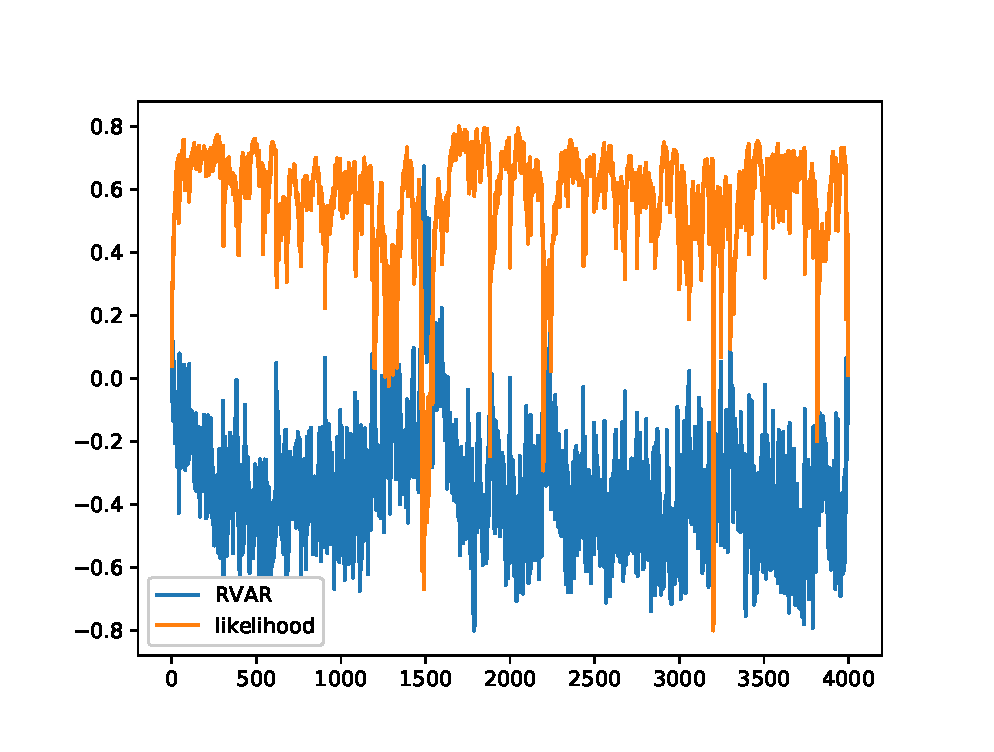
\includegraphics[width=\textwidth]{Plots/likelihood_evolution_1.eps}
    \end{center}
    \caption{The network activation and the corresponding likelihood of the activation for the pre-trained network with a target $\sigma = 1.0$. The correlation of the two series is $-0.59$. The likelihood has been rescaled to the same interval of $[-0.8, 0.8]$ as the series itself. One can clearly see the negative relationship of likelihood and the spikes in the series. Under \textit{normal} conditions, this means in times of low volatility, the likelihood is larger than at times where there is a spike in the series. This is to be expected because spikes are comparably rare and the network has mostly adapted to these low volatility regimes. The edge of the \textit{plasticity experts}, as with the \textit{loss experts}, is expected to be found in the relative likelihood and the networks' reaction to the spikes in the series and their resulting likelihoods.}
    \label{FIG:IBMRVAR}
\end{figure}


\subsection{Predictive Performance}

This section presents the empirical forecasting performance of the plasiticity approach in comparison to benchmark tasks including the HAR model by \cite{Corsi2009}, the exponential weighted experts of Echo State Network and a single Echo State Network with equivalent size and hyperparameter optimization that has been performed for the spectral radius $\rho$ and bias $\bb$.

\begin{table}
\begin{center}
    \begin{tabular}{l|c|c|c|c}
        & initial transient & training & validation & testing \\ \hline
        ESN & $444$ & $2700$ & \multirow{2}{*}{$300$} & \multirow{2}{*}{$1000$} \\
        \cline{1-3}
        HAR & \multicolumn{2}{|c|}{$3144$} & & 
    \end{tabular}
    \label{TABLE:TimeSeriesSplit}
\end{center}
\caption{Split of the timeseries into different parts during the empirical application. The echo state network approaches have an initial transient to wash out the initialization of the network state which - for the convenience of the other sets - was chosen as $444$. As the HAR model doesn't need this transient, those additional days are attributed to the training set which results in a larger training set of $3144$ days.}
\end{table}

The timeseries has been divided according to table \ref{TABLE:TimeSeriesSplit}. The initial transient is referring to the wash-out period of the Echo State Networks to reduce the effect of the 0-initialization of the network state which effectively decreases the training size. This, coming as a tradeoff compared to the HAR model, decreased the amount of data for the estimation because the the validation set was kept the same for the models. The size of the test set, $\hmax$, was set to $1000$ which corresponds to roughly $4$ years of daily data.



\subsubsection{Model Specifications}

Applying the new model, we will compare the following specifications and comparators:
\begin{itemize}
    \item HAR model by \cite{Corsi2009}
    \item ESN experts with loss functions:
    \begin{itemize}
        \item $L(\hat u_t, u_t) = (\hat u_t-u_t)^2$
        \item $L(\hat u_t, u_t) = (\exp{\hat u_t} - \exp{u_t})^2$
        \item $L(\hat u_t, u_t) = \frac{\exp{u_t}^2}{\exp{\hat u_t}^2} - \frac{u_t^2}{\hat u_t^2} - 1$
    \end{itemize} 
    in the exponential update of weights \ref{EQ:LossUpdate}
    \item Plasticity weighted experts with
    \begin{itemize}
        \item $\sigma_k = \frac{1}{\sqrt{2\pi}}$ for all $k = 1, ..., K$
        \item An equally spaced grid of $\sigma_k \in \left[0.8\left(2\pi\right)^{-\frac{1}{2}}, 1.2\left(2\pi\right)^{-\frac{1}{2}}\right]$ around the constant value $\frac{1}{\sqrt{2\pi}}$
    \end{itemize}
    \item Single ESN of comparable size where the hyperparemeter optimzation of the spectral radius $\rho$ and bias $b$ and their validation has been performed using tge same error functions as the experts approach
\end{itemize}
For the loss functions of the loss experts, one has to keep in mind the transformation $u_t = \log{\sqrt{\sigma_t^2}}$ of the timeseries by the square root and the natural logarithm. Hence, the three loss functions correspond to the differnt scales of the series, (i) the logarithm of the volatility $\log{\sigma}$, (ii) the volatility $\sigma$ and (iii) the variance $\sigma^2$.
The choice of $\sigma_k \equiv \frac{1}{\sqrt{2\pi}}$ is motivated by the plasticity update \refp{EQ:Likelihood}, so that the additional factor of $\frac{1}{\sqrt{2\pi\sigma_k^2}} = 1$. All the specifications are trained using the online learning of equations \refp{EQ:RLS1} - \refp{EQ:RLS2}. The choice of the range of spectral radii for the loss experts was motivated by the correspondence to the effective spectral radius of the plasticity experts which are in the range of $[0.8, 1.2]$. This is also supported by the fact that the single ESN with optimized hyperparameters was using a spectral radius of approximately $\rho \in [1.20, 1.25]$, depending on the loss function. Even though, we showed some relationship between the two approaches in section \ref{CH:ExpertModels:Equivalence}, a fair way of comparison still has to be found.


The following results are based on $K=10$ experts, total number of neurons $N=1000$, bias equal to $0.2$. In order to compare the models it is crucial, that the random number generator is fixed for all the applications. When this is neglected, by the nature of the reservoir computing models and their random initalization, the comparison of predictive performance may be due to the state of the random number generator when initializing the random connections and can actually not be attributed to the model design. This way, it can be guaranteed that the differences in performance can be attributed to the different weighting approaches and model specifications.
Beyond the random initialization, the networks of the \textit{plasticity experts} have been adapted to their targeted output distributions using $50$ epochs of presenting them the whole training data set.

The original scale of daily realized volatility was $[0.0032, 0.1142]$ which was log transformed to $[-5.7300, -2.1691]$. For the reservoir computing models, it was finally rescaled to $[-0.8, 0.8]$.


\begin{table}
    \begin{center}
        \begin{tabular}{|c|c|c|c|c|}
            \hline
            \multicolumn{2}{|c|}{}    & spectral radius & bias & regularization \\\hline
            \parbox[t]{2mm}{\multirow{3}{*}{\rotatebox[origin=c]{90}{Single}}} & logMSE & $1.0107$ & $0.4507$ & $20.7$ \\
            \cline{2-5}
            & MSE & $0.8142$ & $0.3711$ & $20.7$ \\
            \cline{2-5}
            & QLIKE & $0.8263$ & $0.8414$ & $6.2$ \\\hline
            \parbox[t]{2mm}{\multirow{3}{*}{\rotatebox[origin=c]{90}{Loss}}} & logMSE  & \multirow{3}{*}{$[0.2, 2.0]$} & \multirow{3}{*}{$0.2$} & $[0.5, 1.8]$  \\
            \cline{2-2}\cline{5-5}
            & MSE & & & $[0.0003, 1.8]$ \\
            \cline{2-2}\cline{5-5}
            & QLIKE & & & $[0.0003, 0.5]$ \\\hline
            \parbox[t]{2mm}{\multirow{2}{*}{\rotatebox[origin=c]{90}{Plast}}} & Constant & $[0.32, 1.51]$ & $[-31.2, 73.4]$ & $[0.5, 1.8]$ \\
            \cline{2-5}
            & Grid & $[0.31, 1.36]$ & $[-33.8, 67.0]$ & $[0.5, 1.8]$ \\
            \hline
        \end{tabular}
        \label{TABLE:SelectedHyperparameters}
    \end{center}
    \caption{Selected hyperparameters of the models based on the training dataset. For the plasticity experts, the spectral radius and the bias are referring to the effective quantities of the network dynamics after tuning them by the plasticity approach.}
\end{table}

The selected hyperparameters are presented in table \ref{TABLE:SelectedHyperparameters}. The highest and lowest values of the spectral radius and bias have been realized for the same networks, which means that there are some extreme networks and some less extremely modified network dynamics. The strong regularization in the Single ESN is to be expected given the larger size of $N = 1000$ neurons, compared to the experts that are only of size $N=100$, but the regularization of the QLIKE is comparably low at $6.2$ but may be attributed to the different combination of a lower spectral radius and a higher bias.




\subsubsection{Fixed Training Performance}
\label{CH:EmpiricalResults:Fixed}

This section presents the out-of-sample predictive performance of the models referring to section \ref{CH:Application:Forecasting:Fixed} where the models have only been trained on the training set, which is up to $\ttrain = 3444$, and have not been re-estimated for the predictions.

\begin{figure}
    \begin{center}
        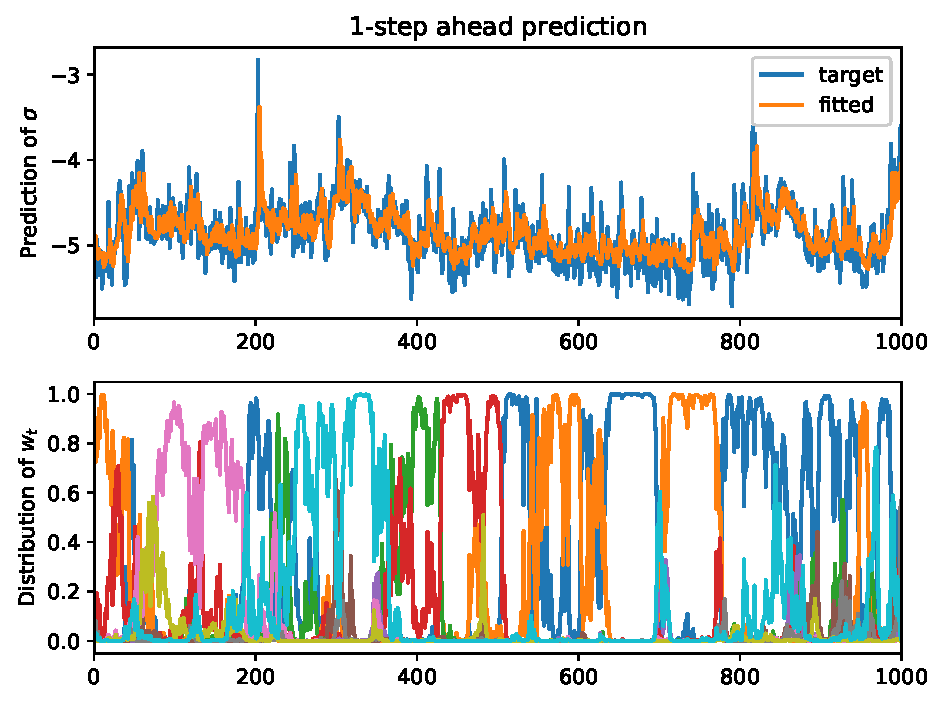
\includegraphics[width=0.45\textwidth]{Plots/Prediction/Experts_logMSE_1step.eps}
        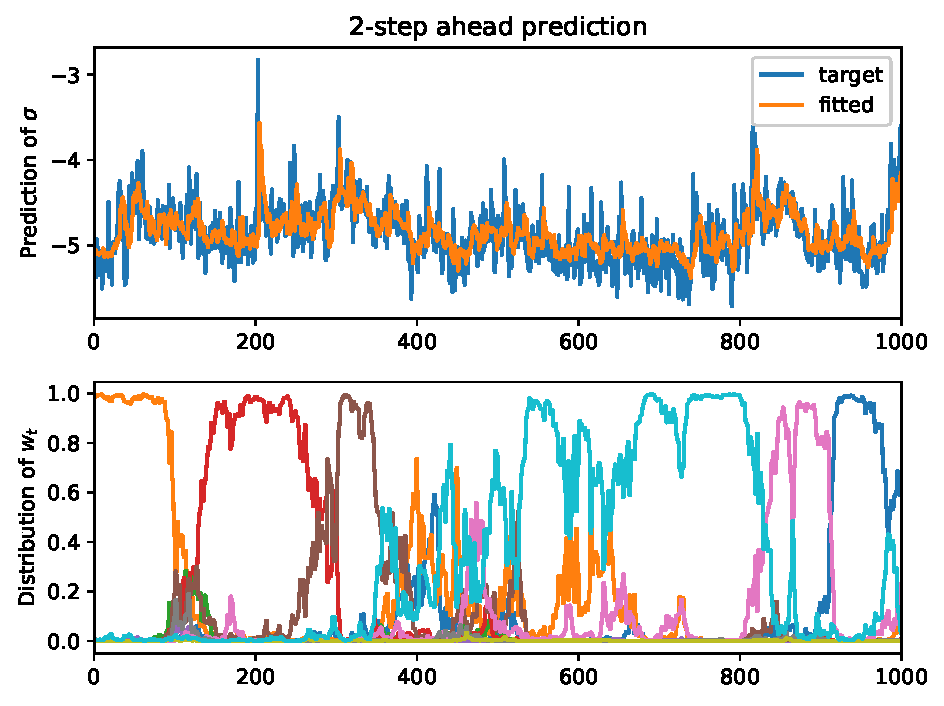
\includegraphics[width=0.45\textwidth]{Plots/Prediction/Experts_logMSE_2step.eps} \\
        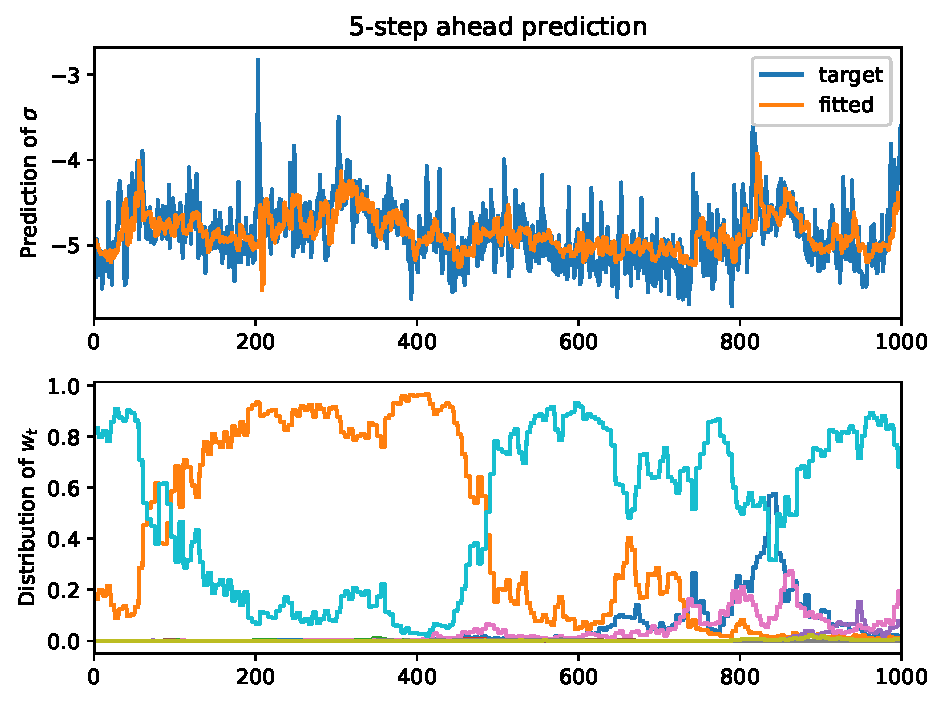
\includegraphics[width=0.45\textwidth]{Plots/Prediction/Experts_logMSE_5step.eps}
        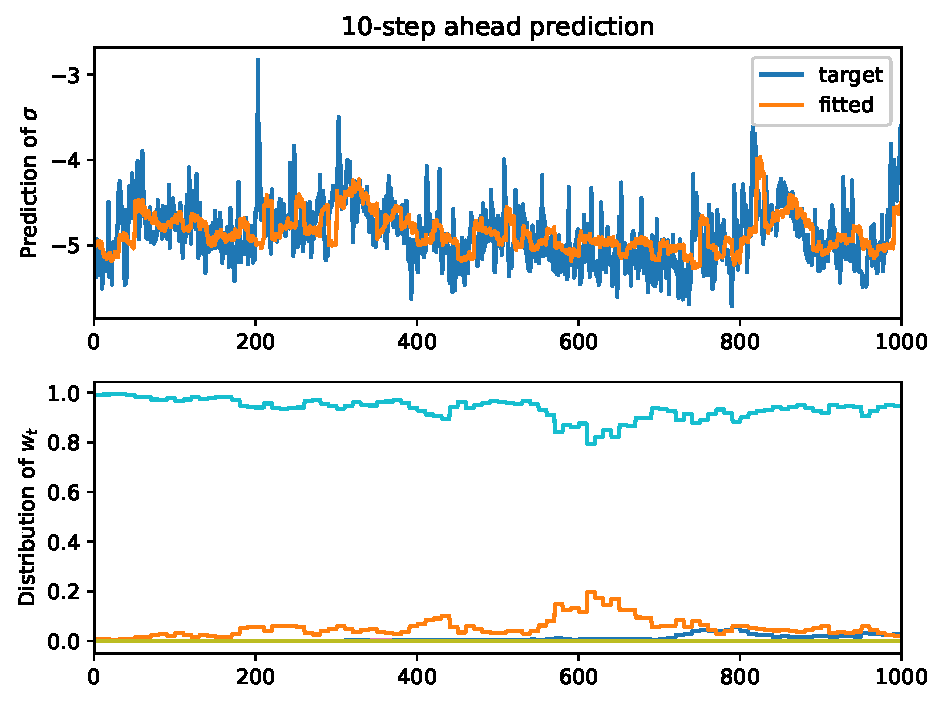
\includegraphics[width=0.45\textwidth]{Plots/Prediction/Experts_logMSE_10step.eps} \\
        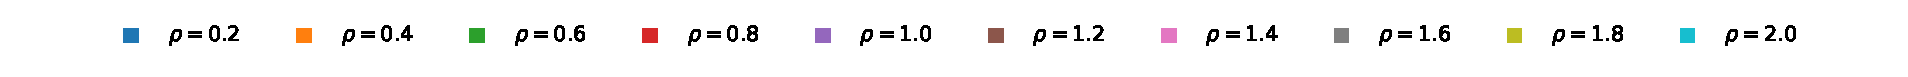
\includegraphics[width=1.0\textwidth]{Plots/Prediction/legend_experts.eps}
        \label{FIG:ExpertsLogMSE}
    \end{center}
    \caption{This is the \textit{loss experts} approach with exponential weighting of the experts based on the mean squared error of the log transformation $\log{\sigma}$. The values of spectral radii are equally space in the interval $\rho \in [0.2, 2.0]$. The networks have only been trained once on the training set as outlined in section \ref{CH:Application:Forecasting:Fixed}.}
\end{figure}

\begin{figure}
    \begin{center}
        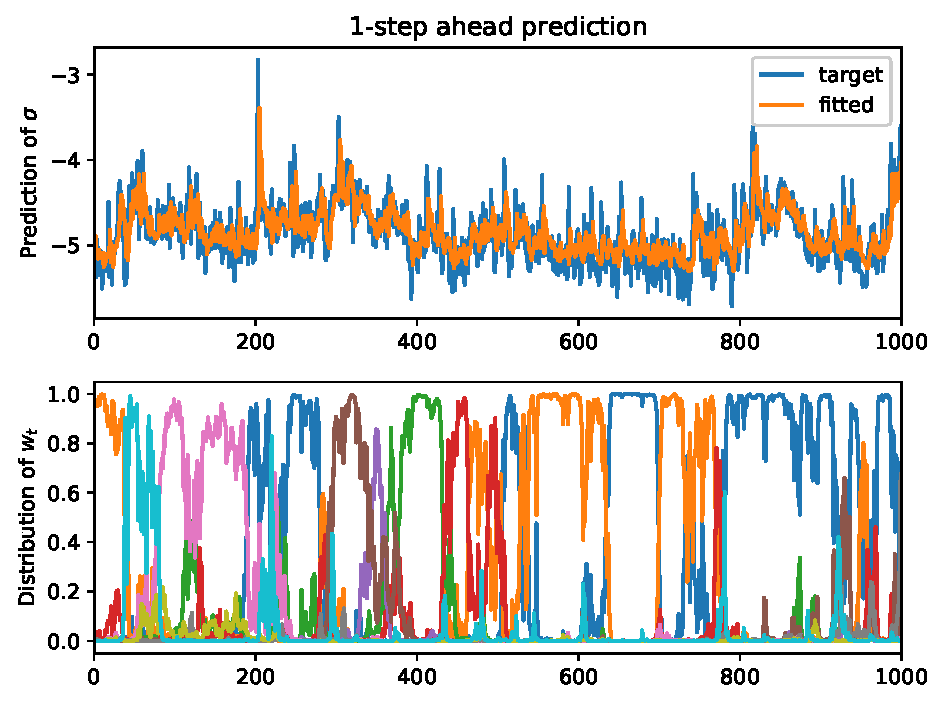
\includegraphics[width=0.45\textwidth]{Plots/Prediction/Experts_MSE_1step.eps}
        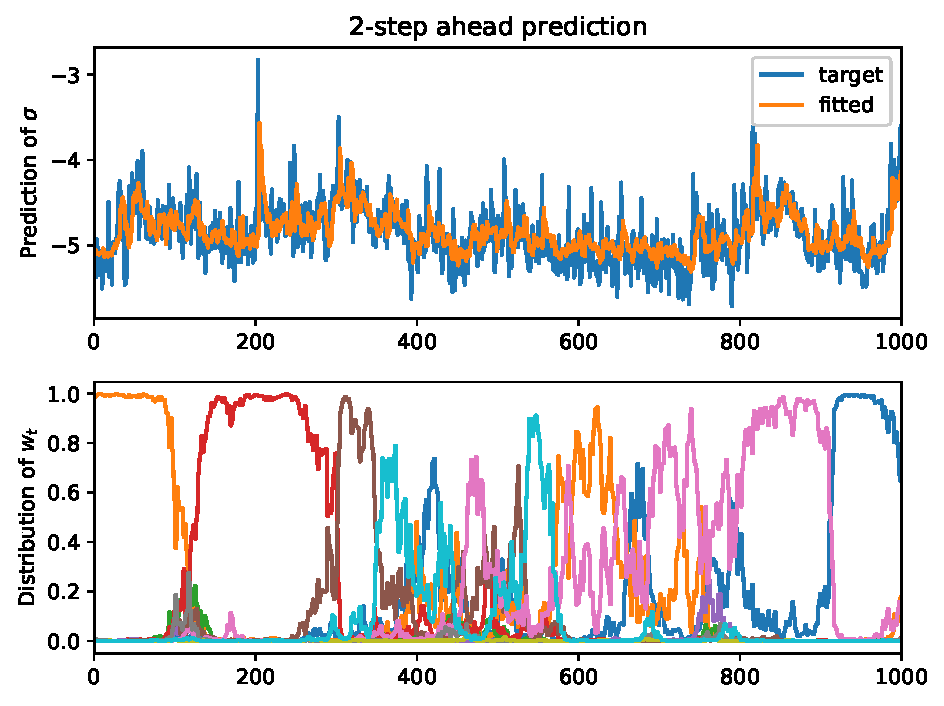
\includegraphics[width=0.45\textwidth]{Plots/Prediction/Experts_MSE_2step.eps} \\
        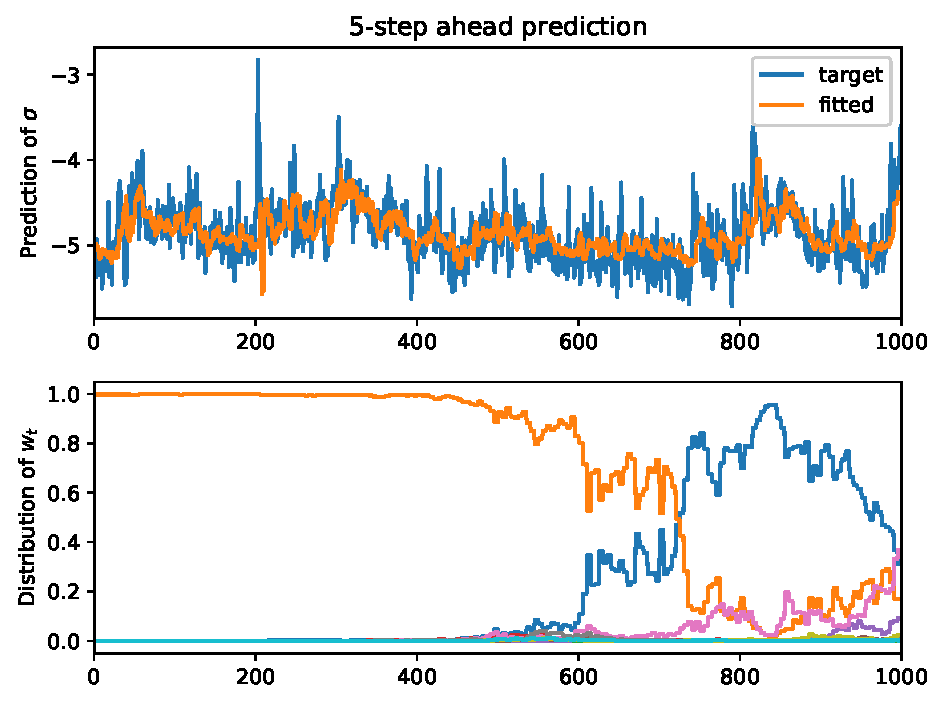
\includegraphics[width=0.45\textwidth]{Plots/Prediction/Experts_MSE_5step.eps}
        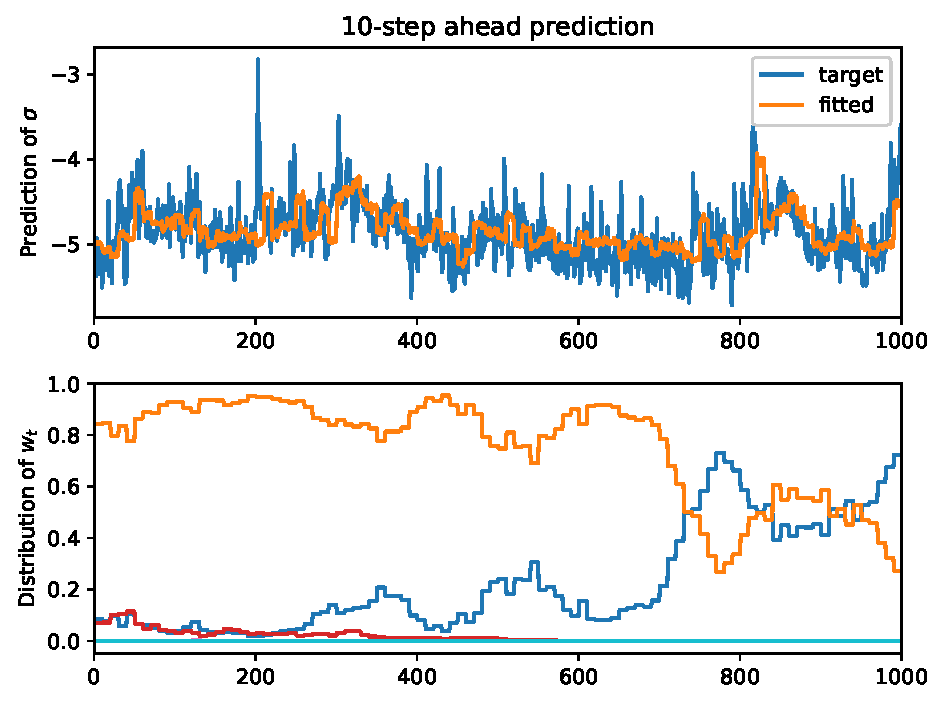
\includegraphics[width=0.45\textwidth]{Plots/Prediction/Experts_MSE_10step.eps} \\
        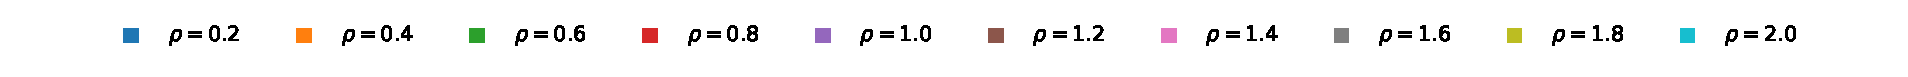
\includegraphics[width=1.0\textwidth]{Plots/Prediction/legend_experts.eps}
        \label{FIG:ExpertsMSE}
    \end{center}
    \caption{This is the \textit{loss experts} approach with exponential weighting of the experts based on the mean squared error of the original time series, so $\sigma$. The values of spectral radii are equally space in the interval $\rho \in [0.2, 2.0]$. The networks have only been trained once on the training set as outlined in section \ref{CH:Application:Forecasting:Fixed}.}
\end{figure}

\begin{figure}
    \begin{center}
        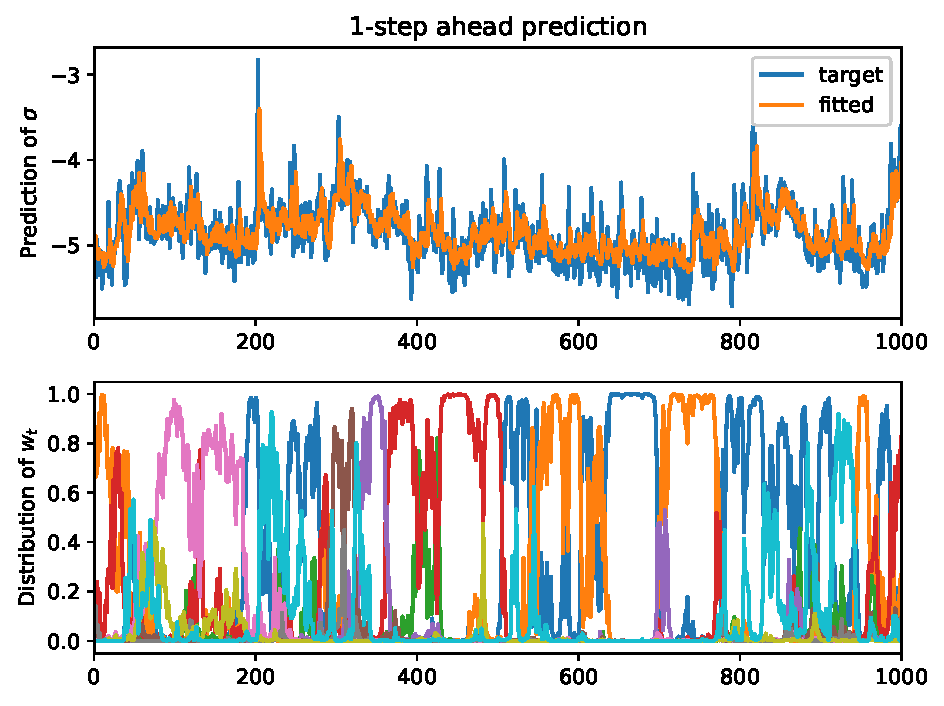
\includegraphics[width=0.45\textwidth]{Plots/Prediction/Experts_QLIKE_1step.eps}
        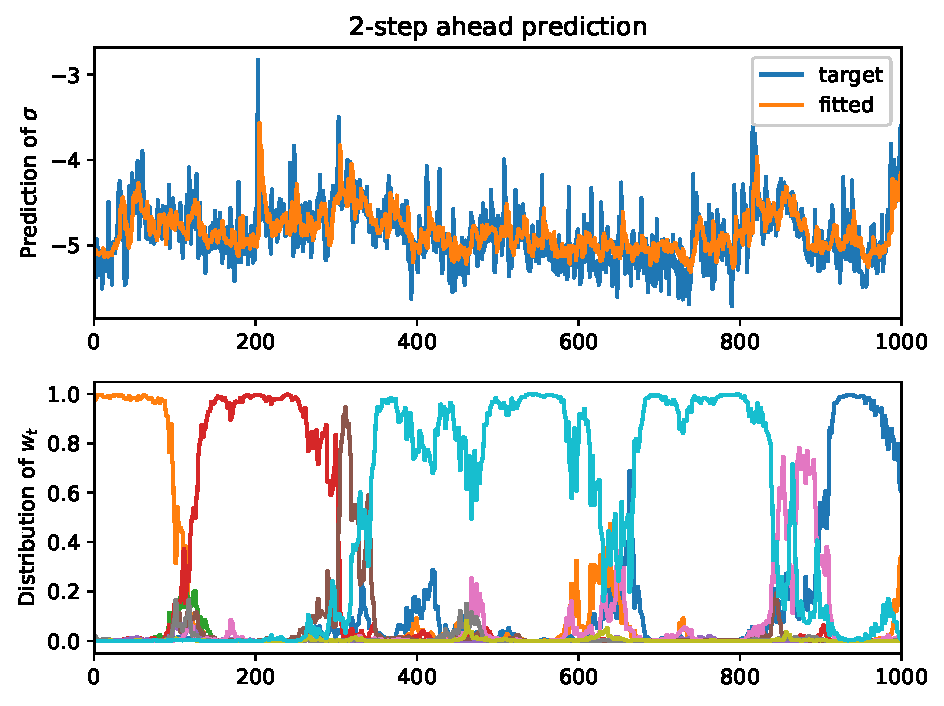
\includegraphics[width=0.45\textwidth]{Plots/Prediction/Experts_QLIKE_2step.eps} \\
        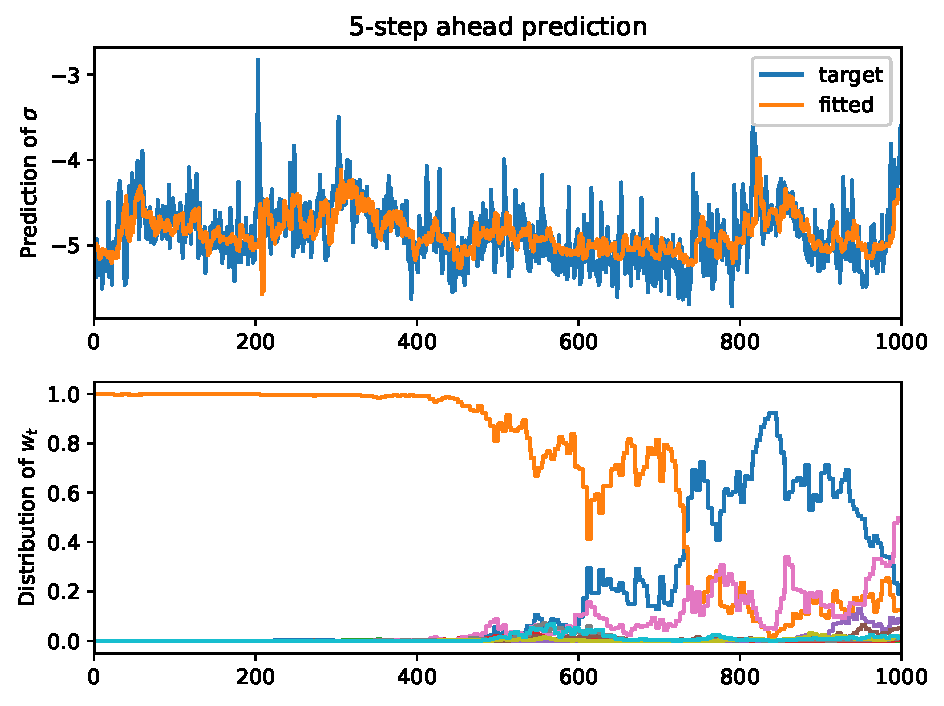
\includegraphics[width=0.45\textwidth]{Plots/Prediction/Experts_QLIKE_5step.eps}
        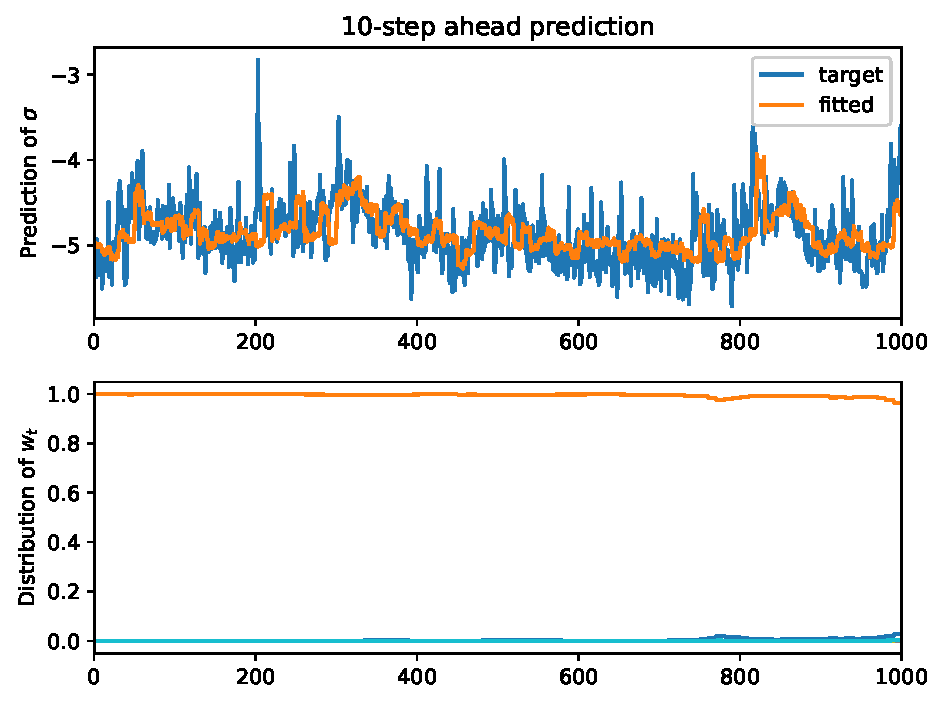
\includegraphics[width=0.45\textwidth]{Plots/Prediction/Experts_QLIKE_10step.eps} \\
        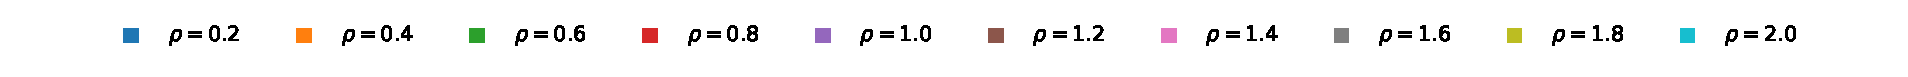
\includegraphics[width=1.0\textwidth]{Plots/Prediction/legend_experts.eps}
        \label{FIG:ExpertsQLIKE}
    \end{center}
    \caption{This is the \textit{loss experts} approach with exponential weighting of the experts based on the QLIKE loss function, so in the scale of $\sigma^2$. The values of spectral radii are equally space in the interval $\rho \in [0.2, 2.0]$. The networks have only been trained once on the training set as outlined in section \ref{CH:Application:Forecasting:Fixed}.}
\end{figure}


\begin{figure}
    \begin{center}
        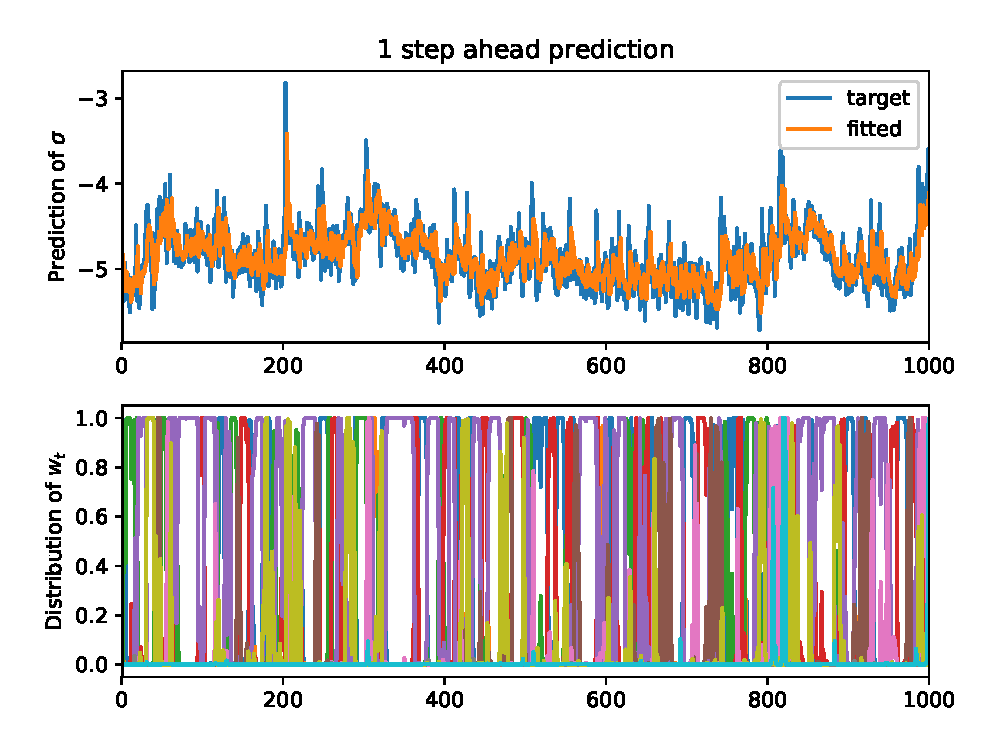
\includegraphics[width=0.45\textwidth]{Plots/Prediction/Plasticity_Constant_1step.eps}
        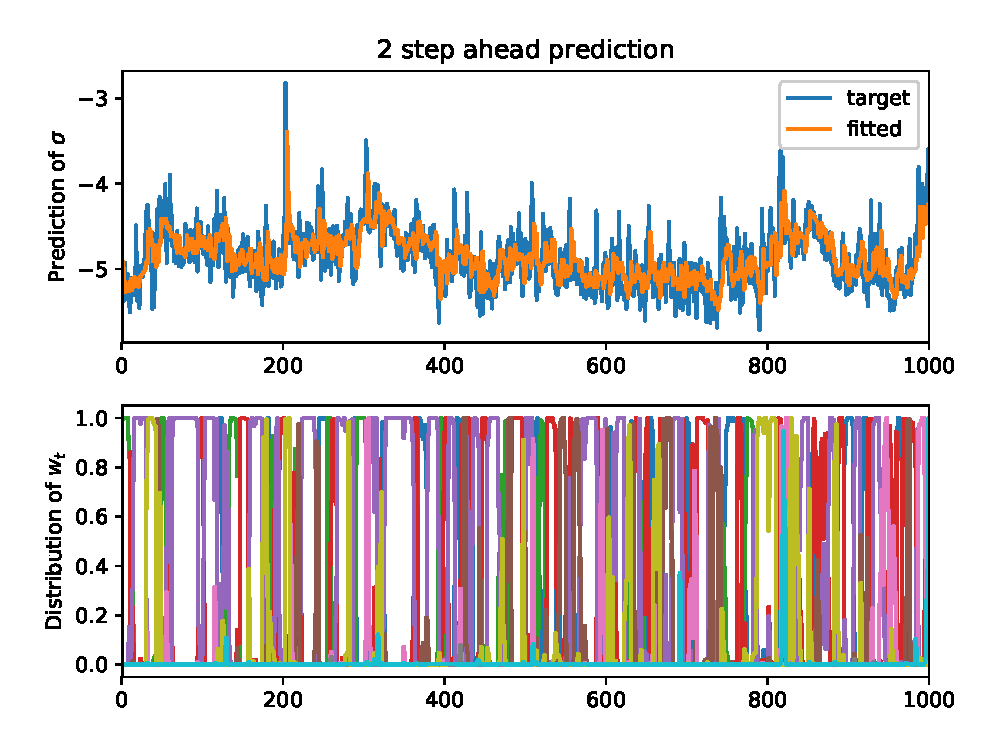
\includegraphics[width=0.45\textwidth]{Plots/Prediction/Plasticity_Constant_2step.eps} \\
        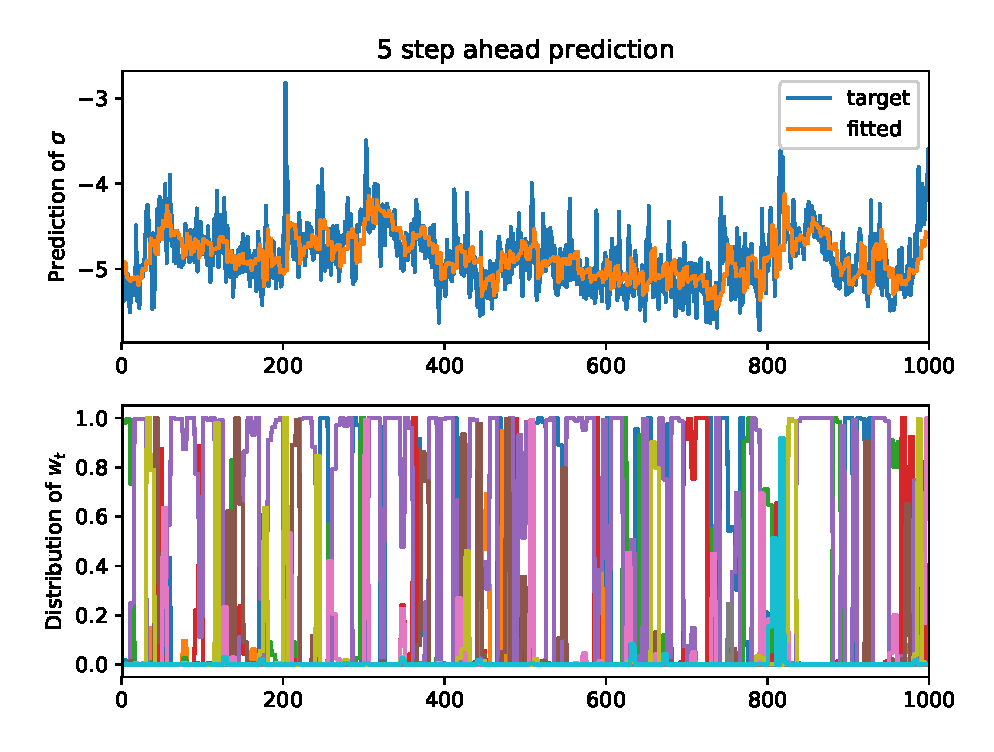
\includegraphics[width=0.45\textwidth]{Plots/Prediction/Plasticity_Constant_5step.eps}
        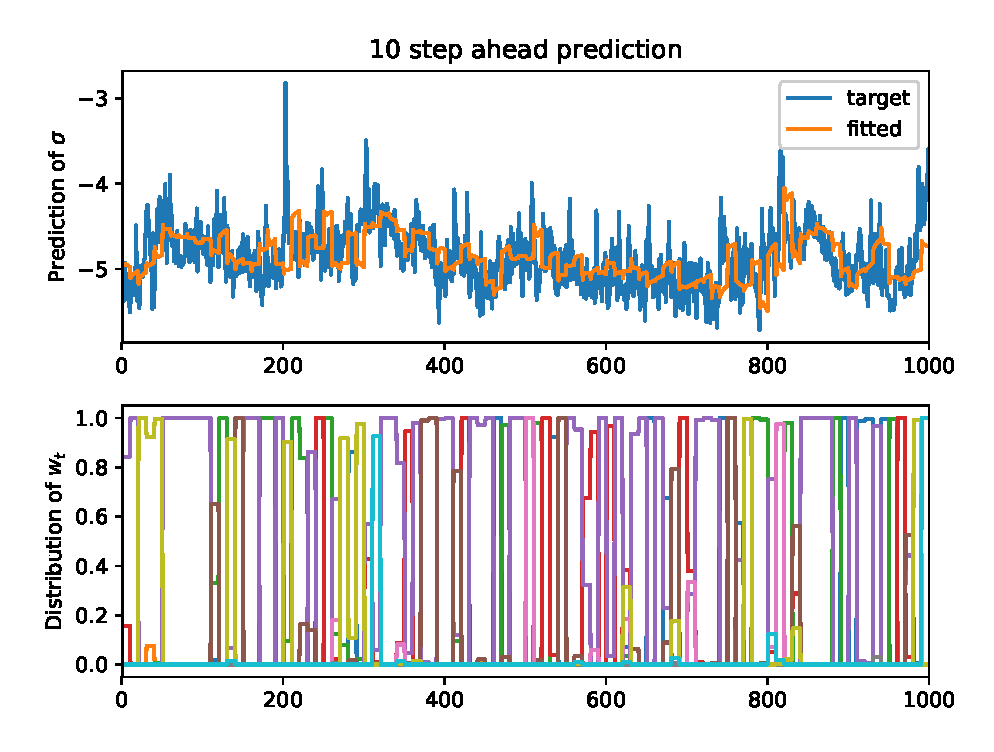
\includegraphics[width=0.45\textwidth]{Plots/Prediction/Plasticity_Constant_10step.eps}
    \end{center}
    \caption{This presents the predictive performance of the \textit{plasticity experts} for 1, 2, 5 and 10 step ahead predictions. The targeted network activations are using a constant $\sigma = \frac{1}{\sqrt{2\pi}}$ for all networks. The networks have only been trained once on the training set as outlined in section \ref{CH:Application:Forecasting:Fixed}.}
    \label{FIG:PlasticityConstant}
\end{figure}

\begin{figure}
    \begin{center}
        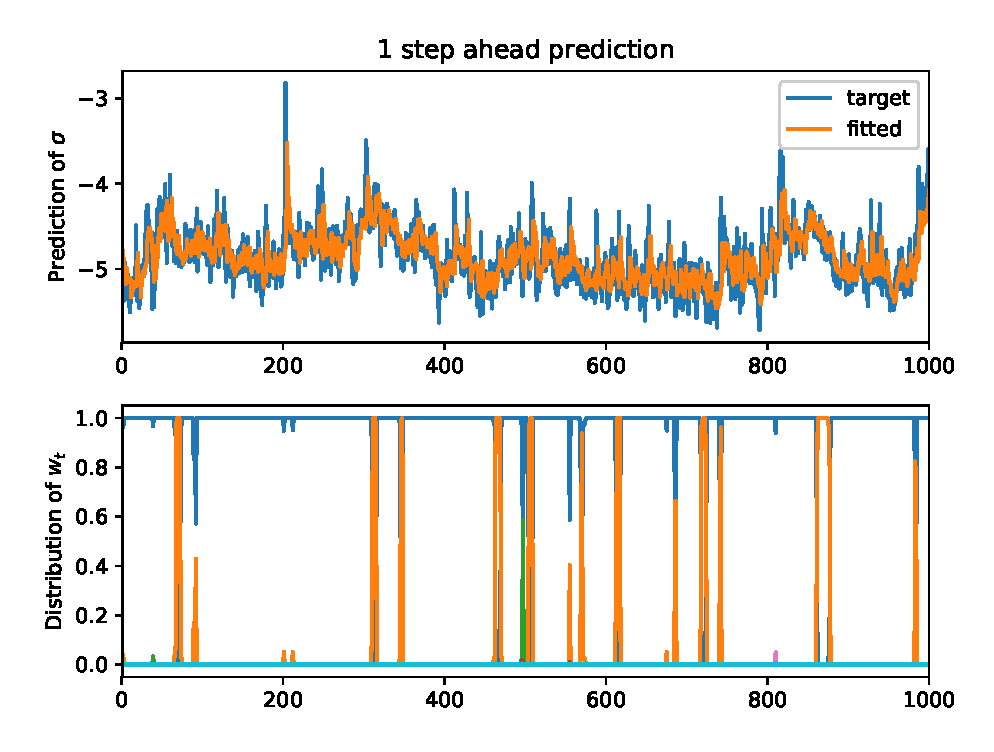
\includegraphics[width=0.45\textwidth]{Plots/Prediction/Plasticity_Grid_1step.eps}
        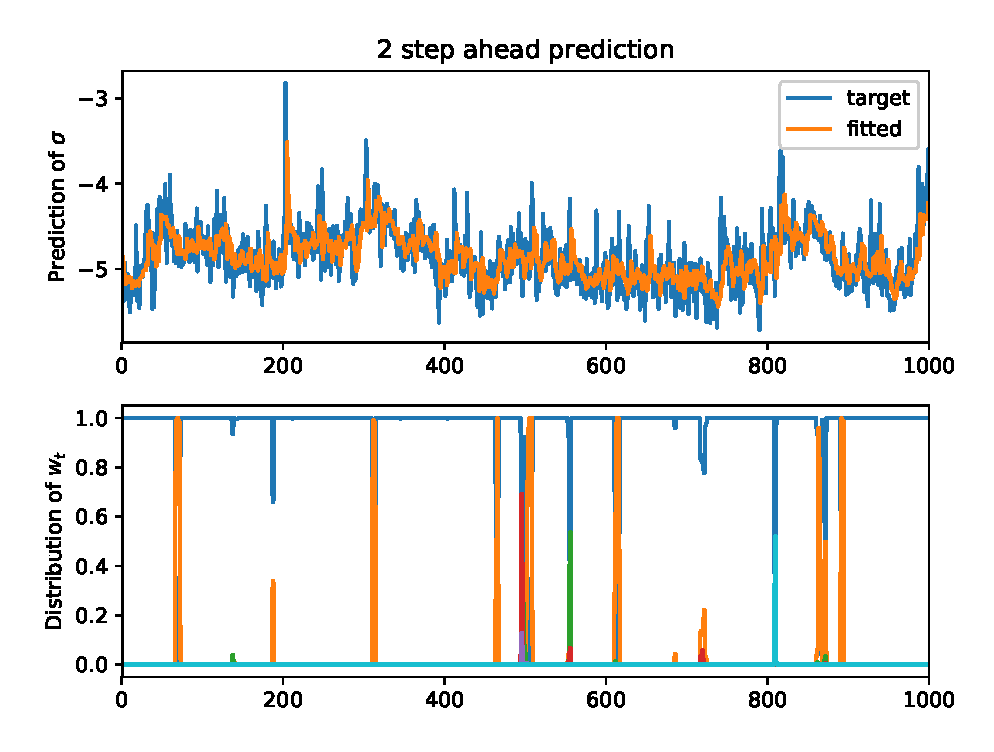
\includegraphics[width=0.45\textwidth]{Plots/Prediction/Plasticity_Grid_2step.eps} \\
        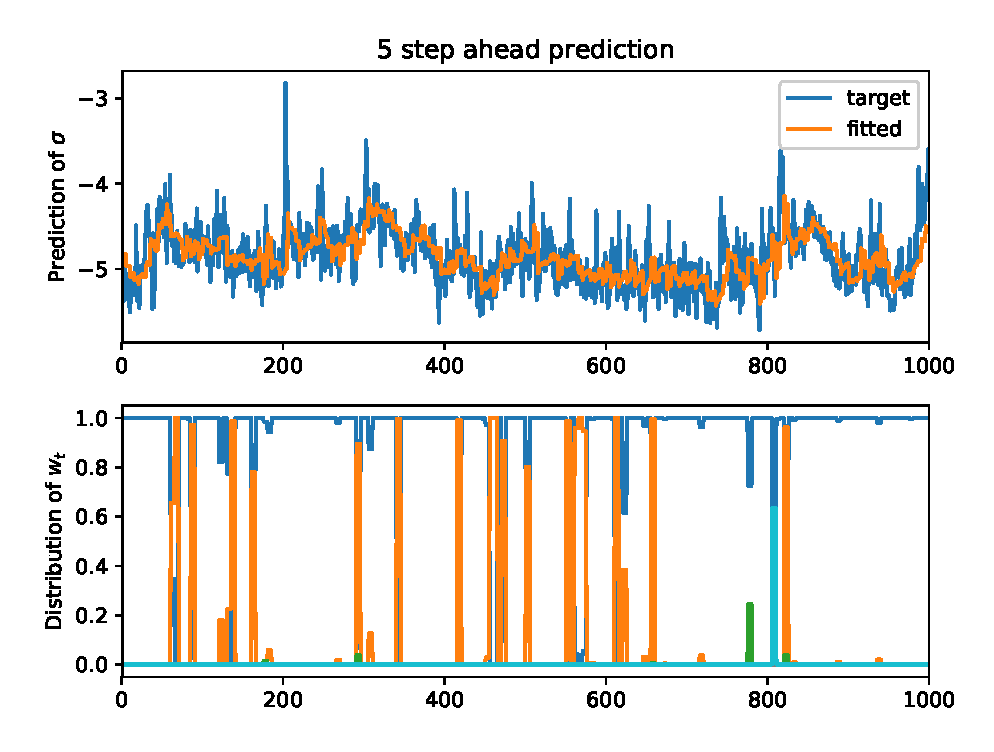
\includegraphics[width=0.45\textwidth]{Plots/Prediction/Plasticity_Grid_5step.eps}
        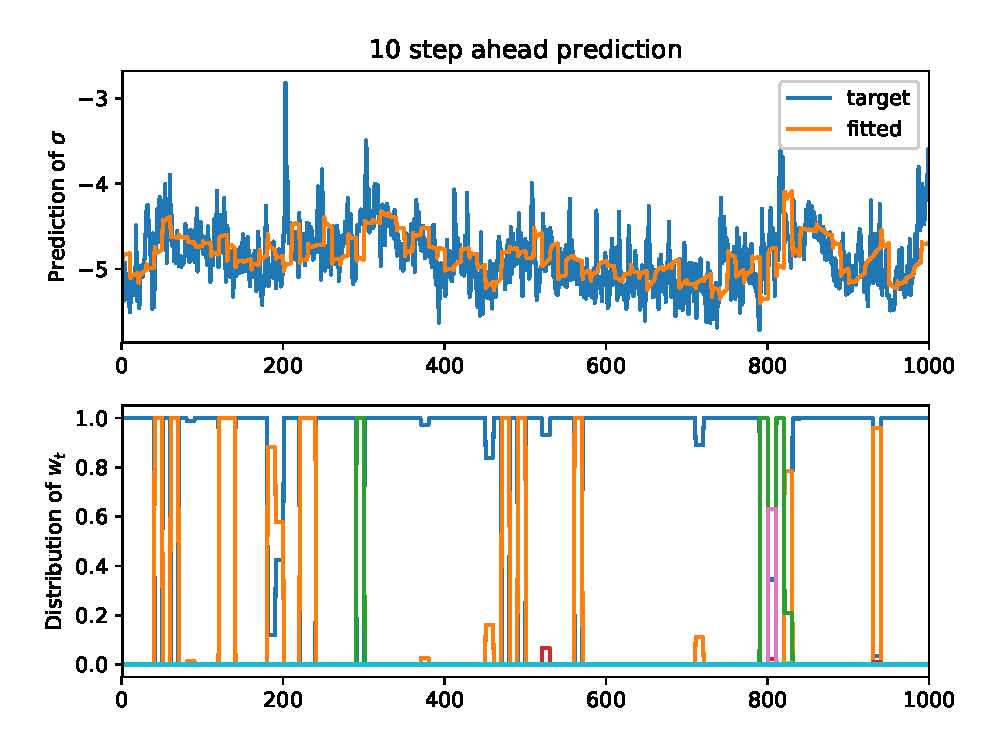
\includegraphics[width=0.45\textwidth]{Plots/Prediction/Plasticity_Grid_10step.eps} \\
        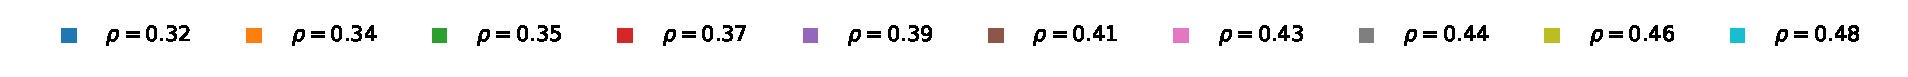
\includegraphics[width=1.0\textwidth]{Plots/Prediction/legend_Grid.eps}
        \label{FIG:PlasticityGrid}
    \end{center}
    \caption{This presents the predictive performance of the \textit{plasticity experts} for 1, 2, 5 and 10 step ahead predictions. The targeted network activations are using an equally spaced grid $\left[0.8\frac{1}{\sqrt{2\pi}}, 1.2\frac{1}{\sqrt{2\pi}}\right]$ around the constant value of $\sigma = \frac{1}{\sqrt{2\pi}}$. The networks have only been trained once on the training set as outlined in section \ref{CH:Application:Forecasting:Fixed}.}
\end{figure}

\begin{figure}
    \begin{center}
        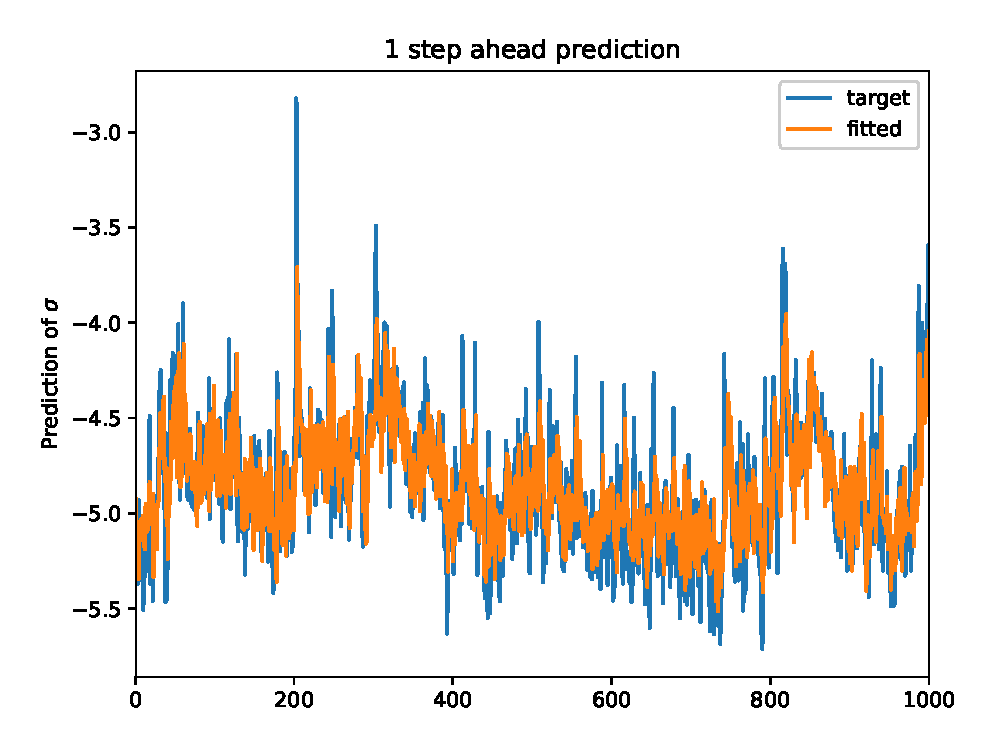
\includegraphics[width=0.45\textwidth]{Plots/Prediction/Single_logMSE_1step.eps}
        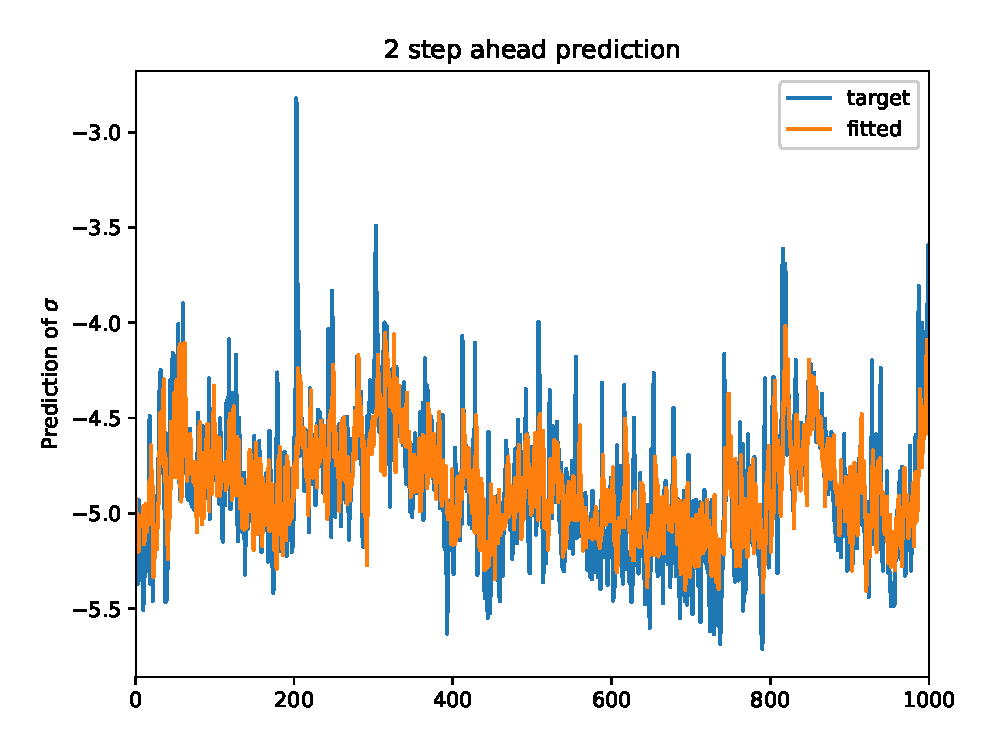
\includegraphics[width=0.45\textwidth]{Plots/Prediction/Single_logMSE_2step.eps} \\
        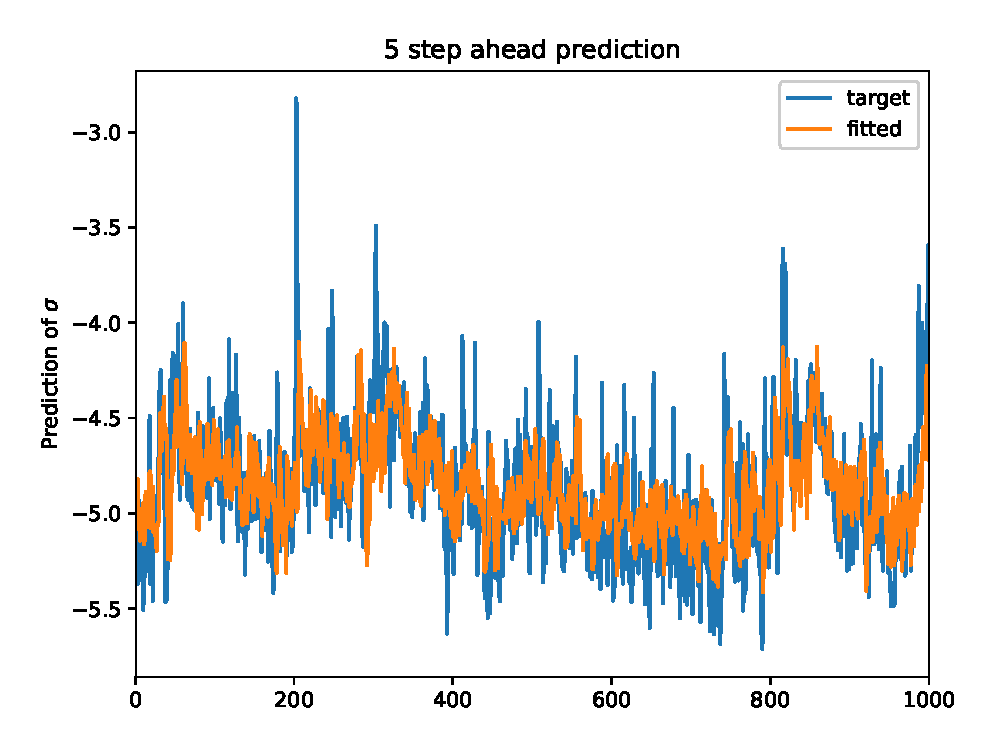
\includegraphics[width=0.45\textwidth]{Plots/Prediction/Single_logMSE_5step.eps}
        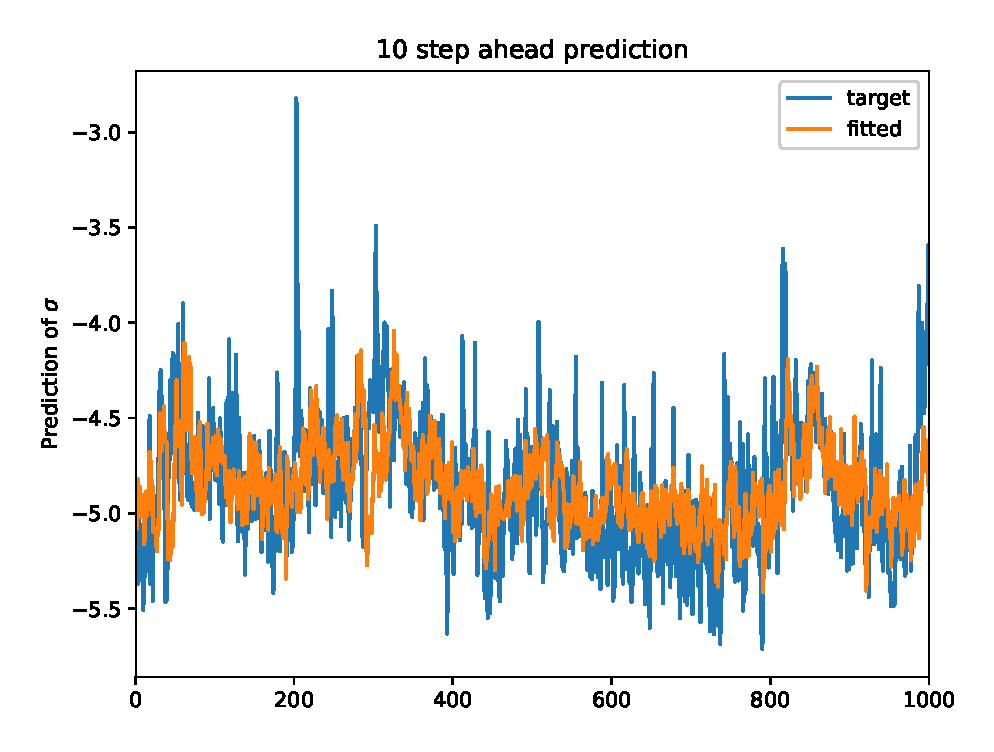
\includegraphics[width=0.45\textwidth]{Plots/Prediction/Single_logMSE_10step.eps}
        \label{FIG:SingleESN}
    \end{center}
    \caption{Single Echo State Network of equivalent size to the experts approach, namely $N=1000$ internal neurons. The hyperparameters that have been tuned for the logMSE are the spectral radius and the bias in the interval $\rho \in (0, 3]$ and bias $b \in [-1,1]$ and using a gradient boosted regression tree from the scikit-optimize package. See the appendix for details on this package.}
\end{figure}


\begin{figure}
    \begin{center}
        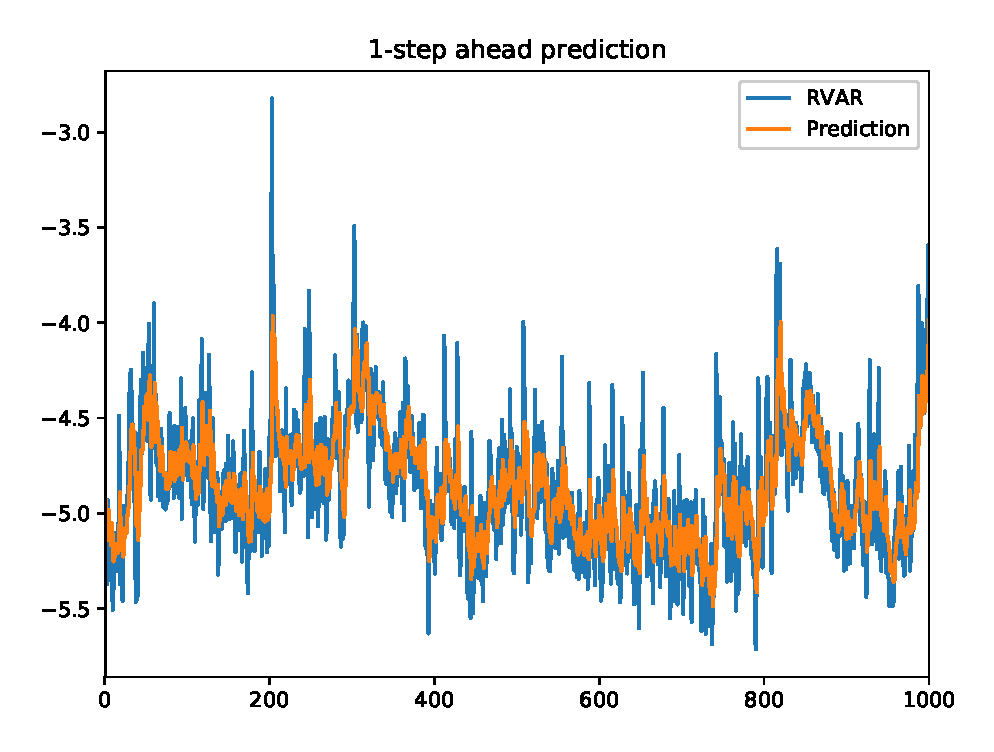
\includegraphics[width=0.45\textwidth]{Plots/Prediction/HAR_1step.eps}
        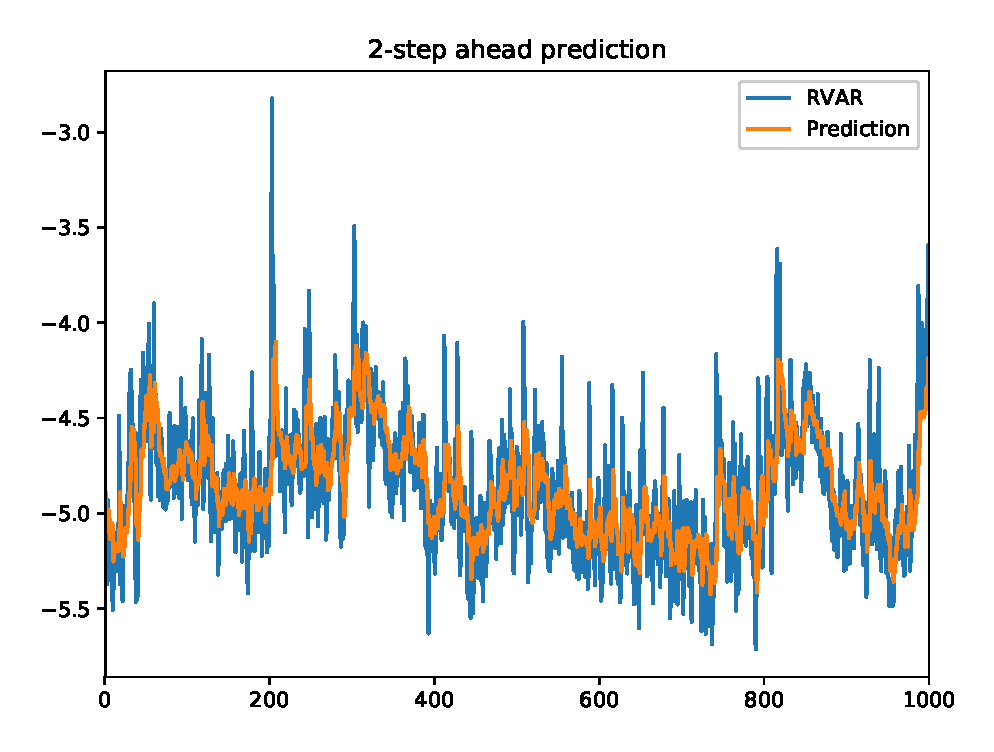
\includegraphics[width=0.45\textwidth]{Plots/Prediction/HAR_2step.eps} \\
        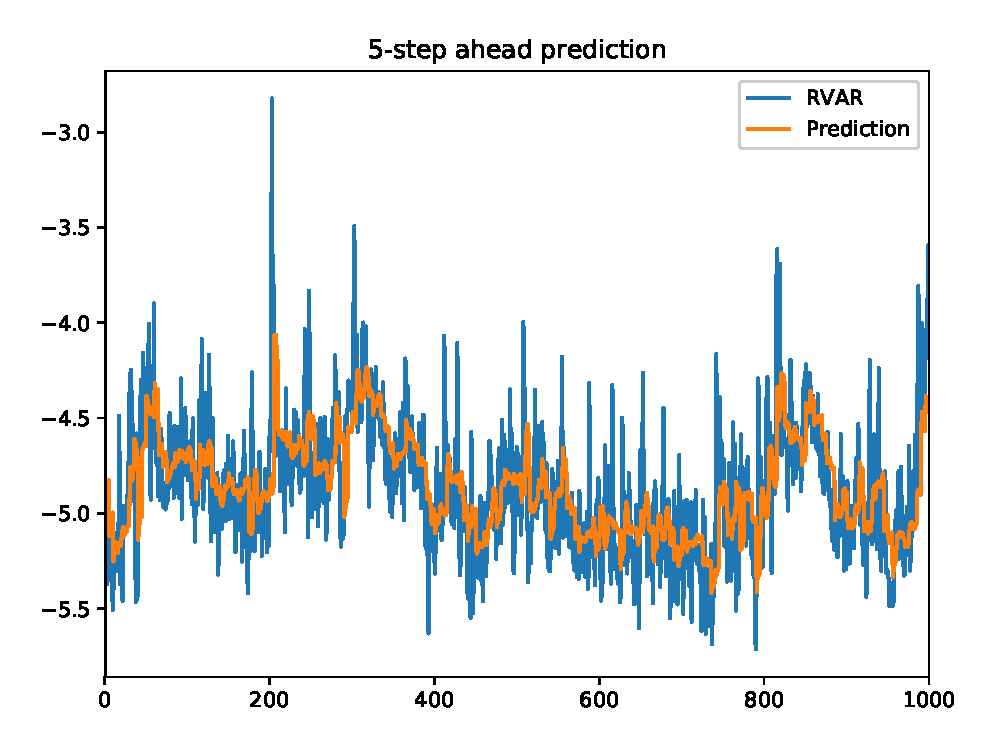
\includegraphics[width=0.45\textwidth]{Plots/Prediction/HAR_5step.eps}
        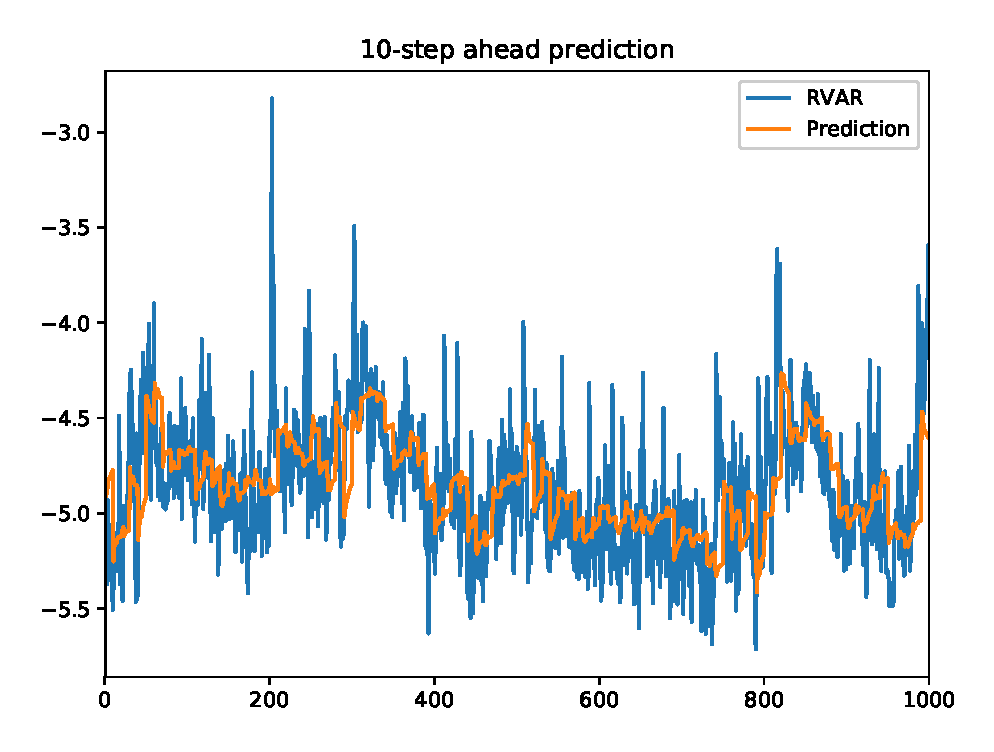
\includegraphics[width=0.45\textwidth]{Plots/Prediction/HAR_10step.eps}
    \end{center}
    \caption{HAR model as proposed by \cite{Corsi2009}, e.g. with daily, weekly and monthly realized volatilities, that has been trained in an online fashion along the lines of recursive least squares \refp{EQ:RLS21}-\refp{EQ:RLS22}.}
    \label{FIG:HAR}
\end{figure}



The figures \ref{FIG:ExpertsLogMSE} to \ref{FIG:HAR} present the predictiven performance of the different models and, in case of the expert methods, the distribution of their weightings over the course of the out-of-sample prediction horizon.
The \textit{loss experts} show a very consistent behaviour for all the error measurements in regards of their weights distribution. There are minor differences but the overall picture of the evolution of the weights stays the same for all apporaches which comes back to the fact that the underlying networks are the same because we fixed the random number generator. Additionally, because the Mean Square Error approach to the weighting showed very little movement when only using equation \refp{EQ:LossUpdate}, the errors for all models were rescaled to $[0,1]$ before applying equation \refp{EQ:LossUpdate} to keep the comparison between the models.
The 1-step ahead prediction is very volatile in terms of the weights which decreases with an increase in the prediction horizon. One can clearly see the dominance of the network with $\rho= 0.2$ in the period from step $500$ to time step $800$ where the series is trending down with little volatility. In the 2-step prediction, the network with the smallest spectral radius of $0.2$ dominates towards the end of the out-of-sample period which is not expected given that the increase in the prediction step would be expected to favor networks with longer memory, so a higher spectral radius. The network with $\rho = 2.0$ is dominating in the mid to end section of the horizon after $\rho = 0.8$ and $\rho = 1.2$ have taken over after $\rho = 0.4$ started the out-of-sample prediction. The weights assigned to networks with smaller spectral radii could be explained by the fact, that the output connections $\wout$ of the networks have not been retrained during the out-ouf-sample prediction and this may be indicative of a regime shift, where the long term dependencies in the series have changed and the prediction is predominantly based on the recent history of the series. On the contrary, there are the 5-step and 10-step ahead predictions. There the networks with the largest spectral radius of $\rho = 2.0$ as gaining weight in the 5-step prediction and and is clearly dominating the 10-step prediction which means that the longer term dependencies are a dominant factor for the predictive ability. Looking at the \textit{loss experts} in figure \ref{FIG:ExpertsMSE} the MSE in the original scale as loss function, the 1-step ahead prediction is still very volatile. The 2-step ahead prediction also shows a very similar picture except that the network with $\rho = 2.0$ is not gaining as much weight as in the log-scale MSE case. The 5-step and 10-step prediction differ significantly. For the original-scale MSE the networks with the lowest spectral radii of $\rho = 0.4$ and $\rho = 0.2$ receive the dominant weights in the beginning and end section of the prediction horizon, respectively.
The QLIKE weighted experts in figure \ref{FIG:ExpertsQLIKE} show a combination of the previous two weighting approaches. Where, still, the 1-step ahead prediction shows its volatile and very similar picture, the 2-step ahead prediction resembles the log-scale MSE distribution of weights and the 5-step and 10-step prediction are more similar to the original-scale MSE weighted experts. The 10-step prediction is even more extrem in the sense, that the network with $\rho = 0.4$ receives a weight of $1$ almost all of the time.

The \textit{plasticity experts} with the same output distributions in figure \ref{FIG:PlasticityConstant} do present a very volatile and quickly adapting behaviour. The similarity between the four panels of figure \ref{FIG:PlasticityConstant} is expected given that after the prediction, the network evolution is corrected by the true series and this is done for all prediction steps. The only difference is the granularity of the weights update which can be seen very well comparing the 1-step and 10-step ahead prediction. The latter behaves like a step function. Additionally, comparing the weights to the experts approach, the distribution of component weights is much more extrem in the sense that the weights mostly alternate between $0$ and $1$ and in rare occasions have a true mixture of components. The similarity of all the panels leads to the conclusion that the empirical distribution and the resulting likelihood of a network's activation can change very quickly. The series and the distribution of the weights, unfortunately, don't seem to correspond in a certain way.
The \textit{plasticity experts} with a grid of output distributions in figure \ref{FIG:PlasticityGrid} on the other hand do present a very different distribution of output weights. Where with constant distributions, most of the networks were involved in the prediction at one point in time, the two experts with the lowest volatility distributions of $\sigma = 0.32$ and $\sigma = 0.34$ make up the resulting predictions. As with the constant plasticity experts the weights alternate between $0$ and $1$ and don't seem to coincide with the series in any remarkable pattern. In very few instances, the networks with $\sigma = 0.35$ and $\sigma = 0.37$ do receive a small weight which is not of long duration\footnote{The values for $\sigma$ don't seem equidistant but this is due to the rounding to two digits.}.

Plots for the predictive performance of the single ESN and the HAR model are provided in figures \ref{FIG:SingleESN} and \ref{FIG:HAR}. The single ESN shows some very choppy behaviour which could indicate an overfitting during the training process. The tuned hyperparemeters of the single ESN are $\rho = 1.2511$ and $b = 0.4406$ \footnote{The bias $b$ is multiplied by $\wbias$ to become $\bb = b \cdot \wbias$.}. The HAR model is in line with expectations. The difference can also be attributed to the fact that the predictions are plotted in the log-scale of $\sigma$. The higher the prediction steps, the calmer the predictions become. Where in the panel of 1-step ahead predictions the forecasts do follow the true series quite strongly this effect decreases with the prediction step and the forecasts have a tendency towards the histrical mean of the series.

For the single ESN, only the prediction of the logMSE related measurements are presented because the chosen hyperparameters were almost the same as the other two error measurements. Out of the three, the logMSE was chosen as it is related to the original scale of the series, namely $\sigma$. The very volatile behaviour of the predictions leads to the concern of overfitting during the training of the network's output connections. This is supported by the fact that the regularization parameter of the ridge regression was chosen on the border of admissible values.

\begin{table}
    \begin{center}
        
\begin{tabular}{l|c|c|c}
Fixed 1-step ahead     & logMSE & MSE $(\times 10^{-5})$ & QLIKE \\\hline
Experts MSE & 0.08758738 & 1.05803697 & 0.24808956\\ 
Experts QLIKE & 0.08760709 & 1.05505096 & 0.24823963\\ 
Experts logMSE & 0.08758126 & 1.05689476 & 0.24847465\\ 
HAR & 0.06847035 & 0.84973355 & 0.19371920\\ 
Plasticity Constant & 0.08933186 & 1.04572311 & 0.25836014\\ 
Plasticity Grid & 0.08640221 & 1.01276597 & 0.25078255\\ 
Single MSE & 0.08334474 & 0.94009009 & 0.20983467\\ 
Single QLIKE & 0.07926708 & 0.93331580 & 0.20988650\\ 
Single logMSE & 0.08267177 & 0.95702170 & 0.22700093\\ 
\end{tabular}
    \end{center}
    \caption{Errors for the prediction for the different models and the $1$-step ahead predictions using a fixed training set as outlined in section \ref{CH:Application:Forecasting:Fixed}.}
    \label{TABLE:1step}
\end{table} 

\begin{table}
    \begin{center}
        
\begin{tabular}{l|c|c|c}
Fixed 2-step ahead     & logMSE & MSE $(\times 10^{-5})$ & QLIKE \\\hline
Experts MSE & 0.08986521 & 1.07277764 & 0.25348541\\ 
Experts QLIKE & 0.09085416 & 1.09143206 & 0.25588969\\ 
Experts logMSE & 0.09084808 & 1.08410217 & 0.25612836\\ 
HAR & 0.07503286 & 0.91231669 & 0.21128034\\ 
Plasticity Constant & 0.08938321 & 1.05612199 & 0.26294063\\ 
Plasticity Grid & 0.08817040 & 1.03261120 & 0.25984234\\ 
Single MSE & 0.08974965 & 1.00270113 & 0.22271637\\ 
Single QLIKE & 0.08679926 & 0.99016069 & 0.23042241\\ 
Single logMSE & 0.09181919 & 1.04655279 & 0.25124330\\ 
\end{tabular}
    \end{center}
    \caption{Errors for the prediction for the different models and the $2$-step ahead predictions using a fixed training set as outlined in section \ref{CH:Application:Forecasting:Fixed}..}
    \label{TABLE:2step}
\end{table}

\begin{table}
    \begin{center}
        
\begin{tabular}{l|c|c|c}
Fixed 5-step ahead     & logMSE & MSE $(\times 10^{-5})$ & QLIKE \\\hline
Experts MSE & 0.09987065 & 1.17159711 & 0.30540002\\ 
Experts QLIKE & 0.09973242 & 1.16626035 & 0.30564940\\ 
Experts logMSE & 0.09832657 & 1.14407191 & 0.30210400\\ 
HAR & 0.08737418 & 1.03945024 & 0.26712508\\ 
Plasticity Constant & 0.09897247 & 1.14413505 & 0.31834281\\ 
Plasticity Grid & 0.09600595 & 1.11135717 & 0.31021388\\ 
Single MSE & 0.10656475 & 1.19625577 & 0.29094670\\ 
Single QLIKE & 0.09785688 & 1.11072290 & 0.28079199\\ 
Single logMSE & 0.10401672 & 1.16531048 & 0.30932509\\ 
\end{tabular}
    \end{center}
    \caption{Errors for the prediction for the different models and the $5$-step ahead predictions using a fixed training set as outlined in section \ref{CH:Application:Forecasting:Fixed}..}
    \label{TABLE:5step}
\end{table}

\begin{table}
    \begin{center}
        
\begin{tabular}{l|c|c|c}
Fixed 10-step ahead     & logMSE & MSE $(\times 10^{-5})$ & QLIKE \\\hline
Experts MSE & 0.10915740 & 1.25883661 & 0.33336069\\ 
Experts QLIKE & 0.11004703 & 1.25491580 & 0.34062729\\ 
Experts logMSE & 0.11021187 & 1.24497983 & 0.33841503\\ 
HAR & 0.10138104 & 1.16342703 & 0.31118643\\ 
Plasticity Constant & 0.11787165 & 1.31586371 & 0.36889776\\ 
Plasticity Grid & 0.11188359 & 1.25658633 & 0.34886447\\ 
Single MSE & 0.12216529 & 1.31975650 & 0.34693690\\ 
Single QLIKE & 0.11271315 & 1.23937364 & 0.32947925\\ 
Single logMSE & 0.11743093 & 1.31681358 & 0.35623439\\ 
\end{tabular}
    \end{center}
    \caption{Errors for the prediction for the different models and the $10$-step ahead predictions using a fixed training set as outlined in section \ref{CH:Application:Forecasting:Fixed}..}
    \label{TABLE:10step}
\end{table}


The tables \ref{TABLE:1step} to \ref{TABLE:10step} present the prediction error for the out-of-sample part of the series, this is the last $1000$ observations, for the different prediction step sizes. 
The error measurements, namely logMSE, MSE and QLIKE are referring to the different scales of $\log{\sigma}$, $\sigma$ and $\sigma^2$, respectively, which is in accordance with the hyperparameters' validation of the \textit{loss experts} and the single ESN.

The HAR model by \cite{Corsi2009} presents the best performance throughout all prediction steps for the logMSE. After the log transformation the volatility process becomes linear and it is to be exptected that the HAR model, which can be regarded as a restricted AR(22) model and therefore is linear, should outperform the other models in this matter. The better performance of the HAR model can also be seen in MSE and in the QLIKE error. This phenomenon can be explained by the fact that the HAR model is by its nature of an AR-process capturing changes in the regime of the time series where the reservoir computing models are only fed the time series itself and don't receive a preprocessed (in the sense of aggregation) of the signal. The only regime change that the HAR model is not able to adapt to is the intercept, but this is also the case for the other models and in comparison the HAR model beats all other models. This will also become clearer in the following section \ref{CH:EmpiricalResults:Rolling}

Comparing the \textit{plasticity experts} and the \textit{loss experts} in the logMSE, the predictive performance of the former is better for the $1$, $2$ and $5$-step ahead prediction and also for the $10$ step prediction when using the grid of targeted output distributions. The $10$-step ahead prediction horizon of the constant plasticities is worse compared to the experts of all loss functions. This tendency mostly continues for the MSE, where the \textit{plasticity experts} outperform the \textit{loss experts} up to the $5$-step prediction but both \textit{plasticity experts}, with constant output distributions and using a grid, are not able to beat the \textit{loss experts} in the MSE.

A comparison between the two plasticity approaches is difficult as the the constant distribution seems to outperform in the logMSE and the MSE for the $5$ and $10$-step prediction, but the grid of distributions seems to be favourable in terms of logMSE and QLIKE for the $1$ and $2$-step prediction setting.

The \textit{loss experts} consistently dominate in the QLIKE where, independent of the prediction step, they outperform all other model specifications.

\subsubsection{Rolling Training Performance}
\label{CH:EmpiricalResults:Rolling}

This section presents the out-of-sample performance for the approach where the training set is shifted into the testing set. This procedure has been outlined in section \ref{CH:Application:Forecasting:Rolling}.


\begin{figure}
    \begin{center}
        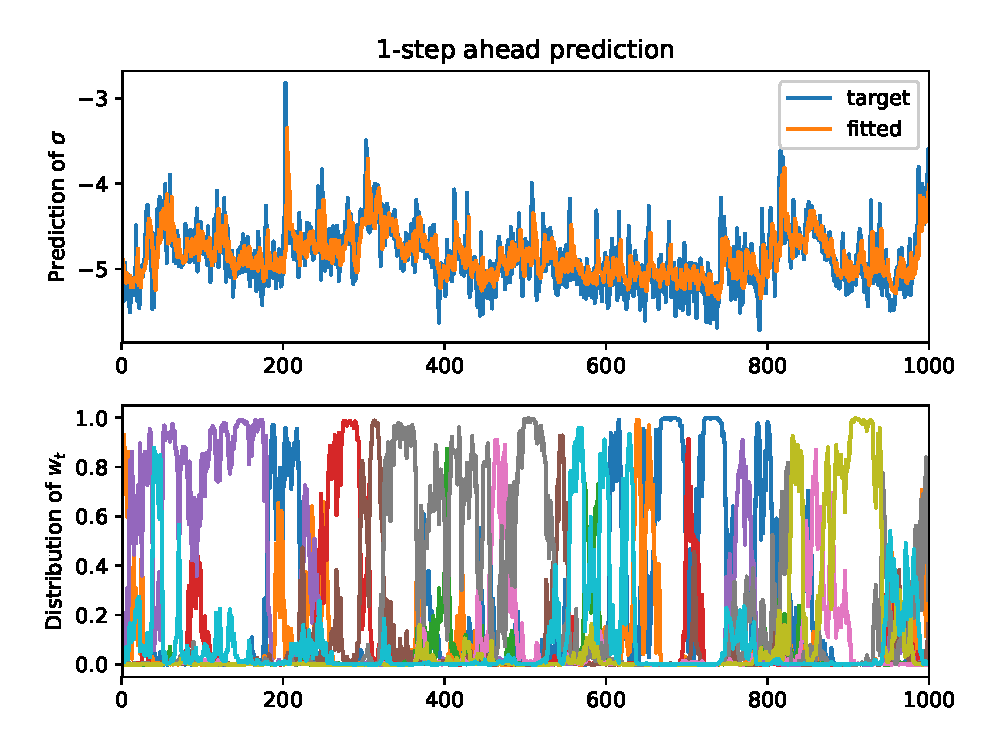
\includegraphics[width=0.45\textwidth]{Plots/Prediction/Experts_logMSE_rolling_1step.eps}
        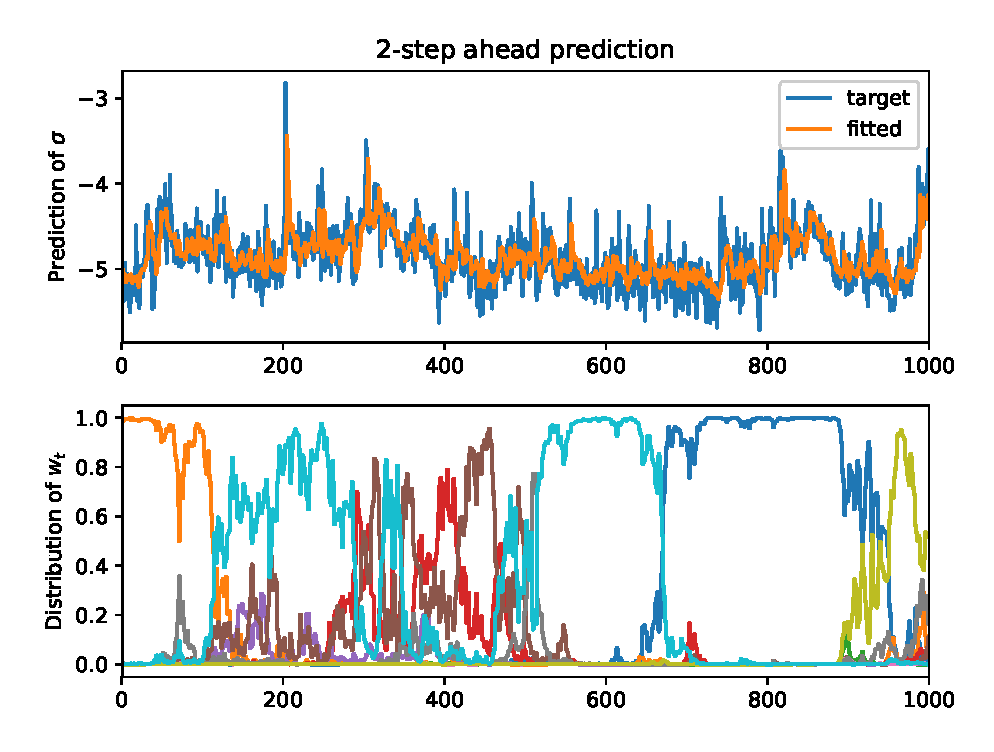
\includegraphics[width=0.45\textwidth]{Plots/Prediction/Experts_logMSE_rolling_2step.eps} \\
        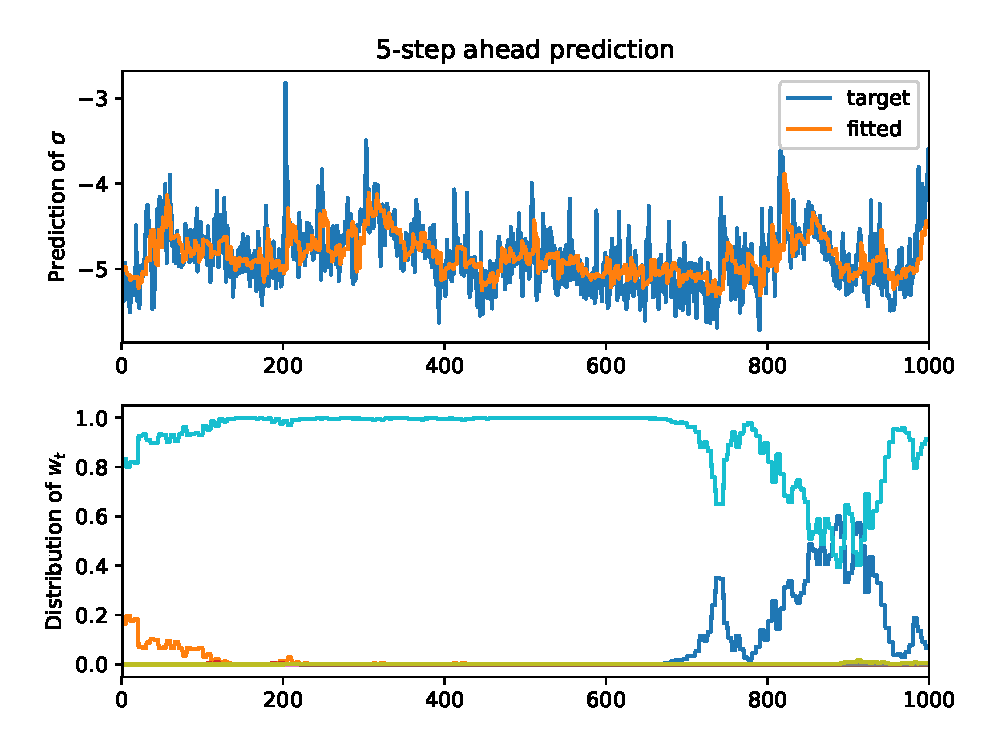
\includegraphics[width=0.45\textwidth]{Plots/Prediction/Experts_logMSE_rolling_5step.eps}
        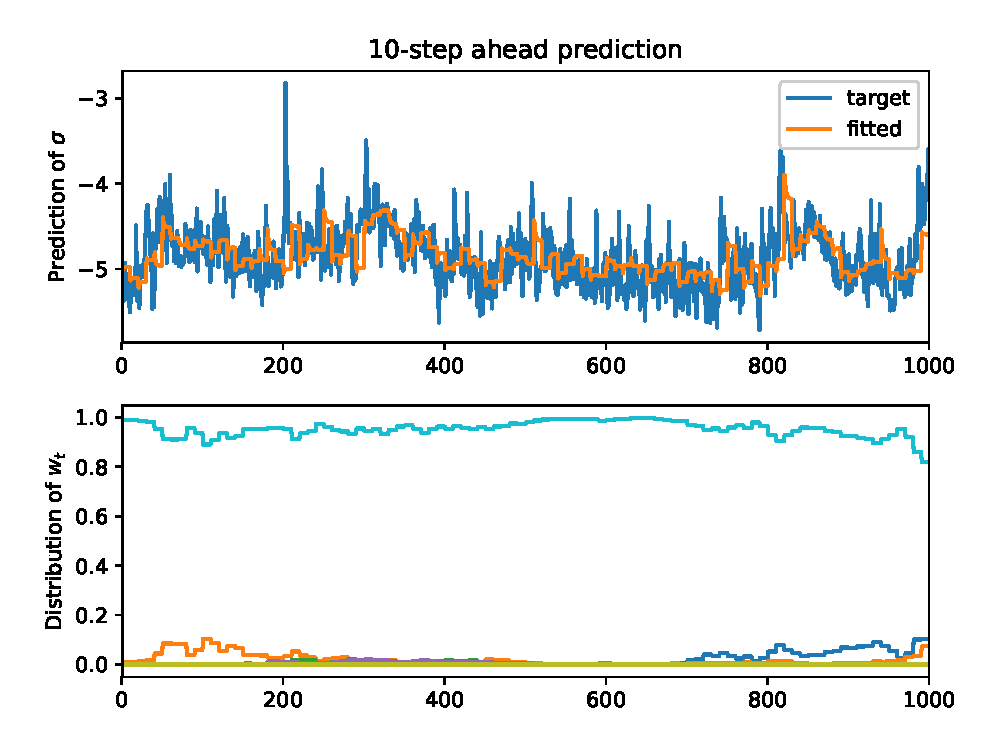
\includegraphics[width=0.45\textwidth]{Plots/Prediction/Experts_logMSE_rolling_10step.eps} \\
        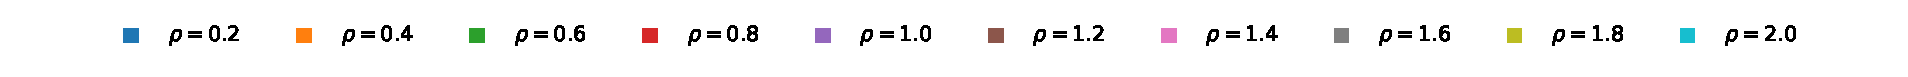
\includegraphics[width=1.0\textwidth]{Plots/Prediction/legend_experts.eps}
        \label{FIG:ExpertsLogMSERolling}
    \end{center}
    \caption{This is the \textit{loss experts} approach with exponential weighting of the experts based on the mean squared error of the log transformation $\log{\sigma}$. The values of spectral radii are equally space in the interval $\rho \in [0.2, 2.0]$. The networks have been retrained in a rolling window fashion as outlined in section \ref{CH:Application:Forecasting:Rolling}.}
\end{figure}

\begin{figure}
    \begin{center}
        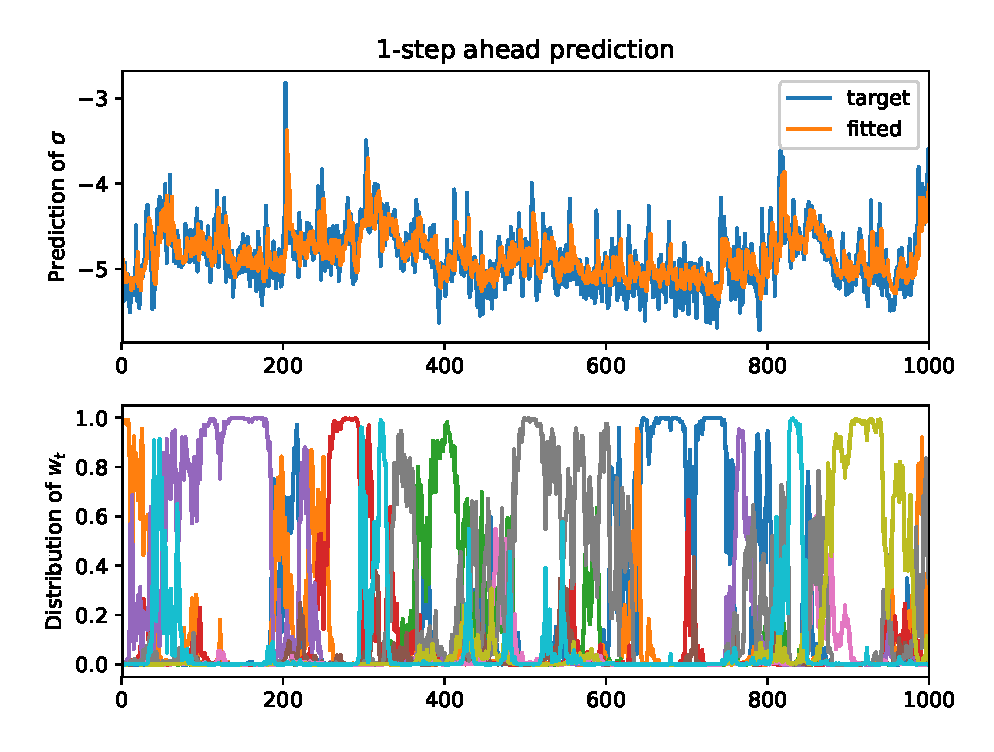
\includegraphics[width=0.45\textwidth]{Plots/Prediction/Experts_MSE_rolling_1step.eps}
        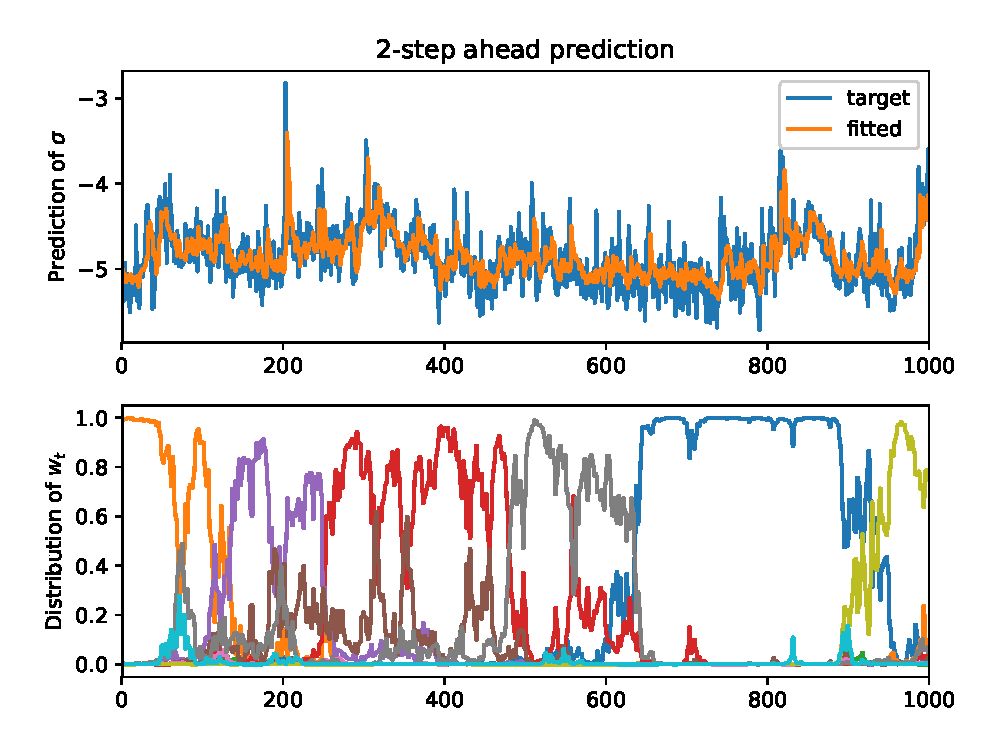
\includegraphics[width=0.45\textwidth]{Plots/Prediction/Experts_MSE_rolling_2step.eps} \\
        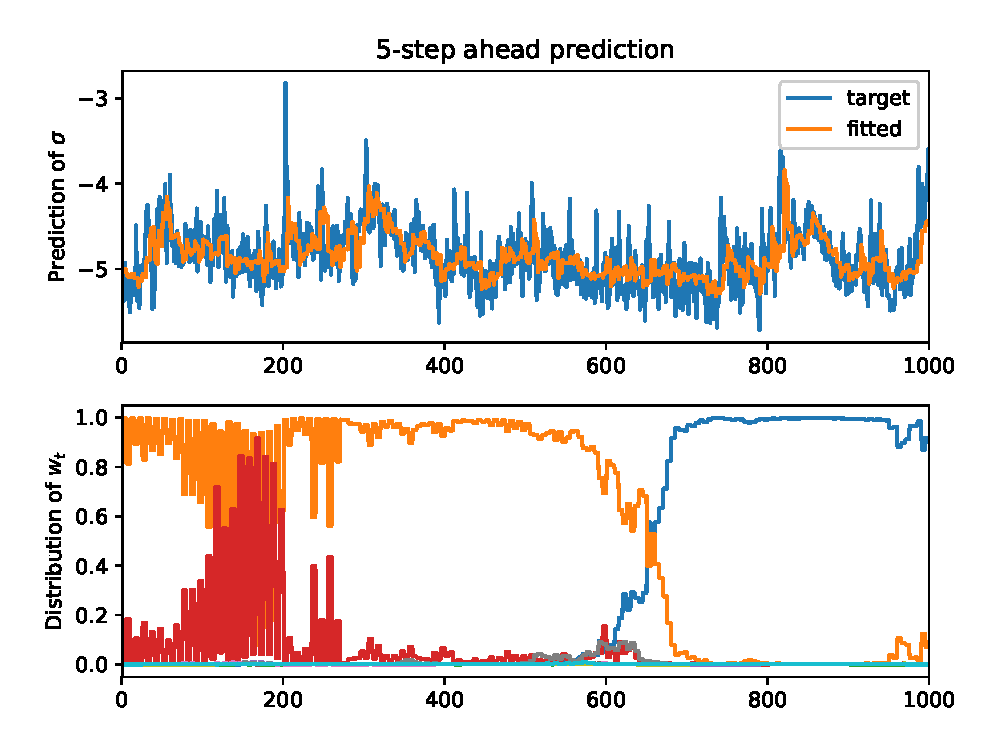
\includegraphics[width=0.45\textwidth]{Plots/Prediction/Experts_MSE_rolling_5step.eps}
        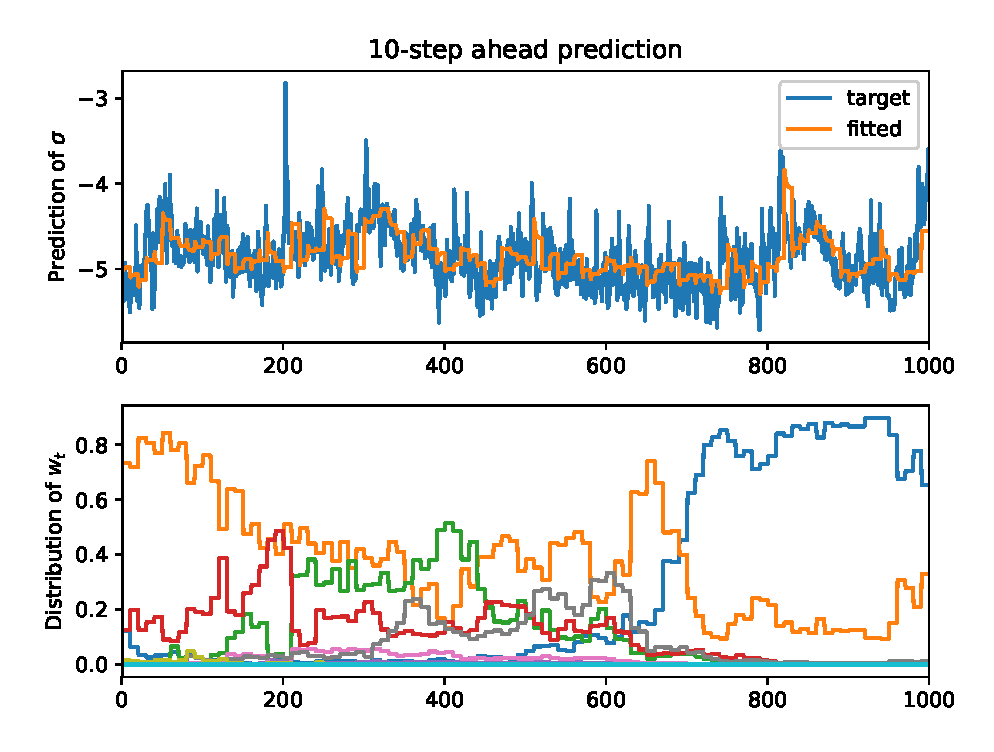
\includegraphics[width=0.45\textwidth]{Plots/Prediction/Experts_MSE_rolling_10step.eps} \\
        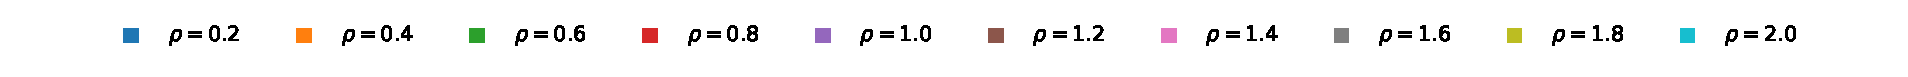
\includegraphics[width=1.0\textwidth]{Plots/Prediction/legend_experts.eps}
    \end{center}
    \caption{This is the \textit{loss experts} approach with exponential weighting of the experts based on the mean squared error of the original time series, so $\sigma$. The values of spectral radii are equally space in the interval $\rho \in [0.2, 2.0]$. The networks have been retrained in a rolling window fashion as outlined in section \ref{CH:Application:Forecasting:Rolling}.}
    \label{FIG:ExpertsMSERolling}
\end{figure}

\begin{figure}
    \begin{center}
        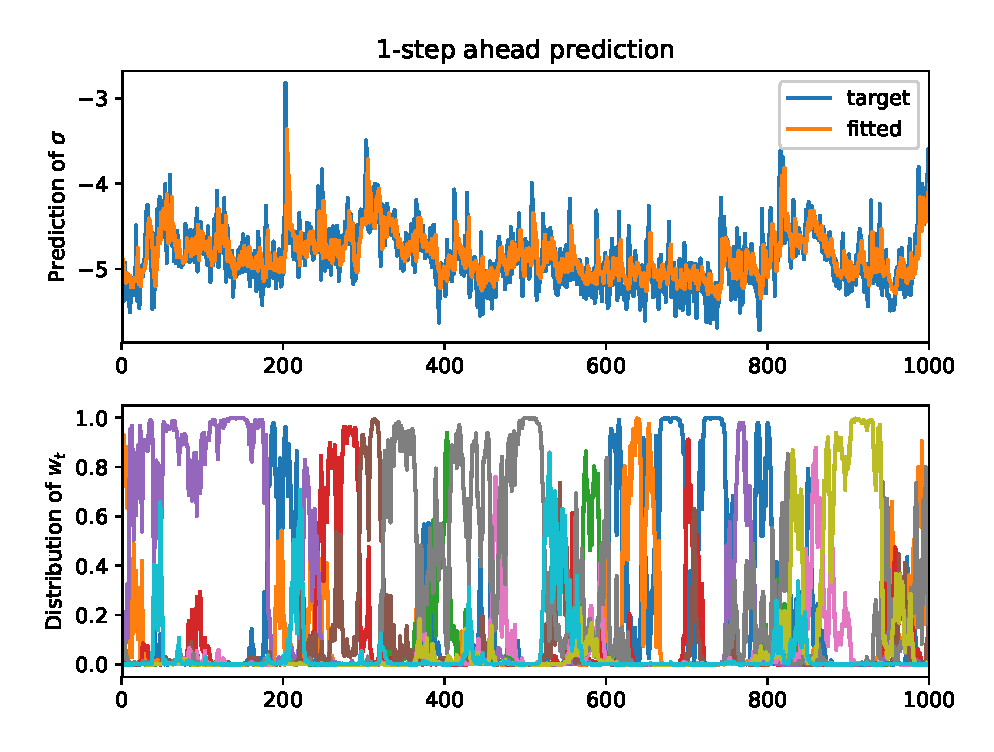
\includegraphics[width=0.45\textwidth]{Plots/Prediction/Experts_QLIKE_rolling_1step.eps}
        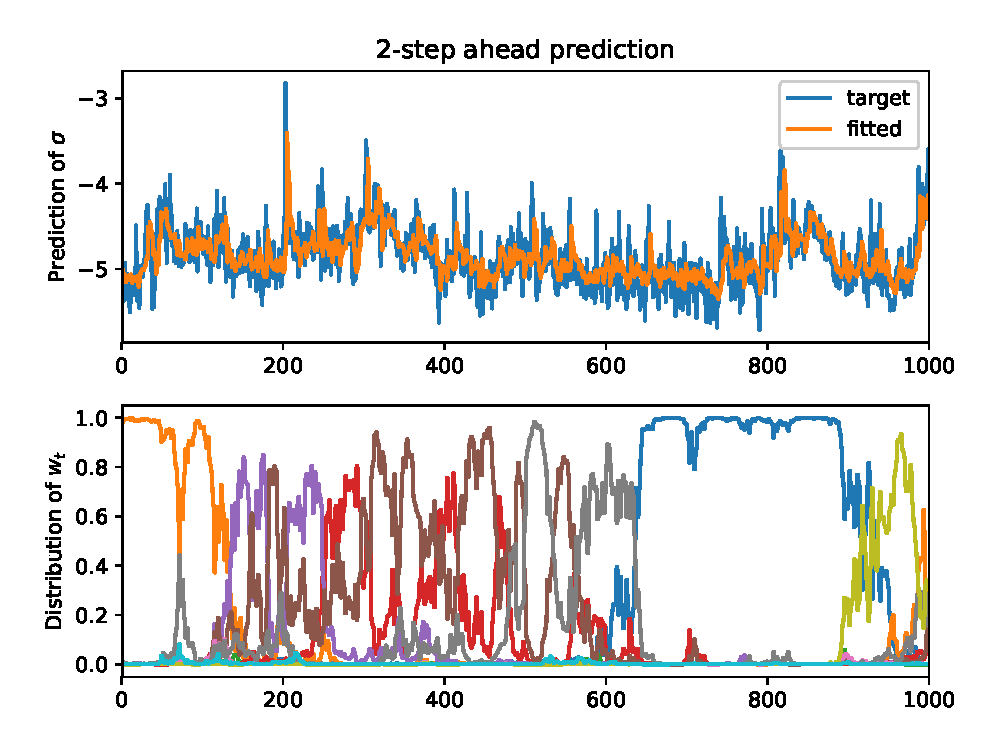
\includegraphics[width=0.45\textwidth]{Plots/Prediction/Experts_QLIKE_rolling_2step.eps} \\
        \includegraphics[width=0.45\textwidth]{Plots/Prediction/Experts_QLIKE_rolling_5step.eps}
        \includegraphics[width=0.45\textwidth]{Plots/Prediction/Experts_QLIKE_rolling_10step.eps} \\
        \includegraphics[width=1.0\textwidth]{Plots/Prediction/legend_experts.eps}
    \end{center}
    \caption{This is the \textit{loss experts} approach with exponential weighting of the experts based on the QLIKE loss function, so in the scale of $\sigma^2$. The values of spectral radii are equally space in the interval $\rho \in [0.2, 2.0]$. The networks have been retrained in a rolling window fashion as outlined in section \ref{CH:Application:Forecasting:Rolling}.}
    \label{FIG:ExpertsQLIKERolling}
\end{figure}


\begin{figure}
    \begin{center}
        \includegraphics[width=0.45\textwidth]{Plots/Prediction/Plasticity_Constant_rolling_1step.eps}
        \includegraphics[width=0.45\textwidth]{Plots/Prediction/Plasticity_Constant_rolling_2step.eps} \\
        \includegraphics[width=0.45\textwidth]{Plots/Prediction/Plasticity_Constant_rolling_5step.eps}
        \includegraphics[width=0.45\textwidth]{Plots/Prediction/Plasticity_Constant_rolling_10step.eps}
    \end{center}
    \caption{This presents the predictive performance of the \textit{plasticity experts} for 1, 2, 5 and 10 step ahead predictions. The targeted network activations are using a constant $\sigma = \frac{1}{\sqrt{2\pi}}$ for all networks. The networks have been retrained in a rolling window fashion as outlined in section \ref{CH:Application:Forecasting:Rolling}.}
    \label{FIG:PlasticityConstantRolling}
\end{figure}

\begin{figure}
    \begin{center}
        \includegraphics[width=0.45\textwidth]{Plots/Prediction/Plasticity_Grid_rolling_1step.eps}
        \includegraphics[width=0.45\textwidth]{Plots/Prediction/Plasticity_Grid_rolling_2step.eps} \\
        \includegraphics[width=0.45\textwidth]{Plots/Prediction/Plasticity_Grid_rolling_5step.eps}
        \includegraphics[width=0.45\textwidth]{Plots/Prediction/Plasticity_Grid_rolling_10step.eps} \\
        \includegraphics[width=1.0\textwidth]{Plots/Prediction/legend_Grid.eps}
    \end{center}
    \caption{This presents the predictive performance of the \textit{plasticity experts} for 1, 2, 5 and 10 step ahead predictions. The targeted network activations are using an equally spaced grid $\left[0.8\frac{1}{\sqrt{2\pi}}, 1.2\frac{1}{\sqrt{2\pi}}\right]$ around the constant value of $\sigma = \frac{1}{\sqrt{2\pi}}$. The networks have been retrained in a rolling window fashion as outlined in section \ref{CH:Application:Forecasting:Rolling}.}
    \label{FIG:PlasticityGridRolling}
\end{figure}

\begin{figure}
    \begin{center}
        \includegraphics[width=0.45\textwidth]{Plots/Prediction/Single_logMSE_rolling_1step.eps}
        \includegraphics[width=0.45\textwidth]{Plots/Prediction/Single_logMSE_rolling_2step.eps} \\
        \includegraphics[width=0.45\textwidth]{Plots/Prediction/Single_logMSE_rolling_5step.eps}
        \includegraphics[width=0.45\textwidth]{Plots/Prediction/Single_logMSE_rolling_10step.eps}
    \end{center}
    \caption{Single Echo State Network of equivalent size to the experts approach, namely $N=1000$ internal neurons. The hyperparameters that have been tuned for the logMSE are the spectral radius and the bias in the interval $\rho \in (0, 3]$ and bias $b \in [-1,1]$ and using a gradient boosted regression tree from the scikit-optimize package. See the appendix for details on this package. The networks have been retrained in a rolling window fashion as outlined in section \ref{CH:Application:Forecasting:Rolling} but hyperparameters have only been optimized on the fixed training set.}
    \label{FIG:SingleESNRolling}
\end{figure}


\begin{figure}
    \begin{center}
        \includegraphics[width=0.45\textwidth]{Plots/Prediction/HAR_rolling_1step.eps}
        \includegraphics[width=0.45\textwidth]{Plots/Prediction/HAR_rolling_2step.eps} \\
        \includegraphics[width=0.45\textwidth]{Plots/Prediction/HAR_rolling_5step.eps}
        \includegraphics[width=0.45\textwidth]{Plots/Prediction/HAR_rolling_10step.eps}
    \end{center}
    \caption{HAR model as proposed by \cite{Corsi2009}, e.g. with daily, weekly and monthly realized volatilities. In line with the Echo State Networks, the HAR model has been retrained in the same rolling window fashion as the reservoir commputing models. Given the size of the dataset, no hyperparameters (e.g. regularization) were needed.}
    \label{FIG:HARRolling}
\end{figure}

Figures \ref{FIG:ExpertsLogMSERolling} to \ref{FIG:ExpertsQLIKERolling} present the performance of the performance of the \textit{loss experts} using the rolling window training. The logMSE trained networks shows a very consistent picture. The weighting in the 1-step ahead predictions is very volatile where almost every network receives significant weight at some point over the testing horizon which leads to the interpretation that those predictions are an interplay of short term moves (smaller $\rho$) and longer term trends (higher $\rho$). In the 2-step head prediction, the weights are not as widely distributed over the networks but mostly assigned to the networks with $\rho = 0.4$ in the very beginning, followed by $\rho = 2.0$ towards the middle and $\rho = 0.2$ dominating the end section of the horizon. $\rho = 1.8$ gains some weight in the very end. The 5-step and 10-step ahead predictions present a clear dominance of $\rho = 2.0$ over most of the horizon for the 5-step and over the whole horizon for the 10-step predictions. This is in line with expectations because a higher $\rho$ signifies a longer memory of the network which is needed for longer out-of-sample predictions.

The broad picture of the weights' distribution is the same for the 1-step and 2-step ahead prediction in the \textit{loss experts} with the MSE as error function. The 1-step ahead prediction shows a very similar picture, but slight differences are recognizable by just eyeballing. The 2-step ahead prediction as well shows a very similar picture, however, the weight of $\rho = 2.0$ that is present in the logMSE seems to have been replaced by the network with $\rho = 1.0$ that gains some weight in the beginning to mid section of the prediction.

Putting the \textit{loss experts} with the QLIKE loss function in contrast with the other two, the results look more in line with the MSE than with the logMSE experts. This makes sense because the scales of $\sigma$ and $\sigma^2$ are more alike compared to the $\log{\sigma}$. Surprisingly, the 1-step and 2-step ahead prediction, as with the MSE, still look similar in the sense, that we find a broad spectrum of networks receiving weight in the 1-step ahead prediction and for the 2-step ahead prediction the networks of $\rho = 0.4$, followed by a mixture of different networks, the network of $\rho = 0.2$ in the end section and $\rho = 1.8$ in the very end of the prediction horizon.
For the 5-step ahead prediction, the network with $\rho = 0.4$ is dominating in the beginning and towards the end, the network with $\rho = 0.2$ is taking over. They again switch roles in the very and it ends with $\rho = 0.4$ as the dominant network. The 10-step ahead prediction is dominated by $\rho = 0.4$ throughout the whole prediction horizon.

The general picture that we have seen in the \textit{loss experts} using MSE and QLIKE suggest that, if we are not in the log-scale, short term moves dominate the predictions of future volatility, which stands in contrast to the logMSE where the network with the highest value of $\rho$, namely the network with $\rho = 2.0$ tended to dominate the longer prediction horizons.


The \textit{plasticity experts} with equal output distributions show a very similar weight distribution compared to the fixed training set. The distribution is still very volatile which makes a direct comparison difficult. 
For the networks with different output distributions, however, the distribution is even more concentrated towards the network with $\sigma = 0.32$. This is the case for all prediction steps. While the network with the second lowest $\sigma = 0.34$ is sporadically and for very short amounts of time gaining some weight in the 1-step ahead prediction, this happens fewer and fewer as the prediction horizon increases. This doesn't seem to coincide with the series at all.
Tests with a different grid of lower values was performed as well but didn't show significant improvements in performance or further insights into the resulting weighting. Analyses are provided in appendix \ref{CH:Appendix:GridSmallerSigma}.

For the HAR model in figure \ref{FIG:HARRolling} we can see a very similar behaviour compared to the fixed training set of figure \ref{FIG:HAR}.




\begin{table}
    \begin{center}
        
\begin{tabular}{l|c|c|c}
Rolling 1-step ahead     & logMSE & MSE $(\times 10^{-5})$ & QLIKE \\\hline
Experts MSE & 0.08802286 & 1.06410393 & 0.24888490\\ 
Experts QLIKE & 0.08808350 & 1.06756442 & 0.24892281\\ 
Experts logMSE & 0.08813920 & 1.06925160 & 0.24909907\\ 
HAR & 0.06836762 & 0.84943039 & 0.19290737\\ 
Plasticity Constant & 0.08742805 & 1.03377312 & 0.25916568\\ 
Plasticity Grid & 0.08620444 & 1.02328620 & 0.25938944\\ 
Single MSE & 0.04375821 & 0.52195032 & 0.09560064\\ 
Single QLIKE & 0.03912077 & 0.50217962 & 0.08570485\\ 
Single logMSE & 0.03968808 & 0.51286353 & 0.08754516\\ 
\end{tabular}
    \end{center}
    \caption{Errors of the rolling window prediction for the different models and the $1$-step ahead predictions.}
    \label{TABLE:1stepRolling}
\end{table} 

\begin{table}
    \begin{center}
        
\begin{tabular}{l|c|c|c}
Rolling 2-step ahead     & logMSE & MSE $(\times 10^{-5})$ & QLIKE \\\hline
Experts MSE & 0.08923483 & 1.09138857 & 0.25424408\\ 
Experts QLIKE & 0.08914354 & 1.08832016 & 0.25355556\\ 
Experts logMSE & 0.08863778 & 1.07198041 & 0.25318178\\ 
HAR & 0.07491863 & 0.91276585 & 0.21032252\\ 
Plasticity Constant & 0.08822185 & 1.04517222 & 0.26429428\\ 
Plasticity Grid & 0.08736104 & 1.04320714 & 0.26452248\\ 
Single MSE & 0.06513711 & 0.70083327 & 0.15331451\\ 
Single QLIKE & 0.05814992 & 0.65169373 & 0.13849141\\ 
Single logMSE & 0.06232936 & 0.69091708 & 0.14581589\\ 
\end{tabular}
    \end{center}
    \caption{Errors of the rolling window prediction for the different models and the $2$-step ahead predictions.}
    \label{TABLE:2stepRolling}
\end{table}

\begin{table}
    \begin{center}
        
\begin{tabular}{l|c|c|c}
Rolling 5-step ahead     & logMSE & MSE $(\times 10^{-5})$ & QLIKE \\\hline
Experts MSE & 0.09729214 & 1.14939778 & 0.30033757\\ 
Experts QLIKE & 0.09713321 & 1.14502098 & 0.29860384\\ 
Experts logMSE & 0.09732349 & 1.13903226 & 0.30362584\\ 
HAR & 0.08724299 & 1.04101105 & 0.26582336\\ 
Plasticity Constant & 0.09802419 & 1.14526361 & 0.31551162\\ 
Plasticity Grid & 0.09590954 & 1.11738107 & 0.30815891\\ 
Single MSE & 0.09332434 & 1.07093848 & 0.26010275\\ 
Single QLIKE & 0.08905669 & 1.02041242 & 0.25948164\\ 
Single logMSE & 0.09239568 & 1.04845941 & 0.27164816\\ 
\end{tabular}
    \end{center}
    \caption{Errors of the rolling window prediction for the different models and the $5$-step ahead predictions.}
    \label{TABLE:5stepRolling}
\end{table}

\begin{table}
    \begin{center}
        
\begin{tabular}{l|c|c|c}
Rolling 10-step ahead     & logMSE & MSE $(\times 10^{-5})$ & QLIKE \\\hline
Experts MSE & 0.11097113 & 1.27168492 & 0.34156865\\ 
Experts QLIKE & 0.11154794 & 1.28125508 & 0.34201162\\ 
Experts logMSE & 0.11092033 & 1.25180105 & 0.34742392\\ 
HAR & 0.10088391 & 1.15992706 & 0.30959814\\ 
Plasticity Constant & 0.11459149 & 1.30729493 & 0.36355034\\ 
Plasticity Grid & 0.10688234 & 1.20814290 & 0.34068571\\ 
Single MSE & 0.10229432 & 1.13029632 & 0.29080090\\ 
Single QLIKE & 0.10515565 & 1.17085258 & 0.31481402\\ 
Single logMSE & 0.11414491 & 1.26265779 & 0.35273585\\ 
\end{tabular}
    \end{center}
    \caption{Errors of the rolling window prediction for the different models and the $10$-step ahead predictions.}
    \label{TABLE:10stepRolling}
\end{table}

In terms of prediction errors which are presented in the tables \ref{TABLE:1stepRolling} to \ref{TABLE:10stepRolling}, the stellar performance of the HAR model compared to the reservoir computing models which we have seen in the previous section, decreases. For the rolling 1-step and 2-step ahead prediction, the single ESNs, independent of the associated error function, outperform the HAR model in all measurements. In the 5-step and 10-step ahead predictions, the comparison of the Single ESN and the HAR model depends on the error measurement as well as the hyperparameter tuning of the Single ESN.

Generally, the performance of the \textit{loss experts}, the \textit{plasticity experts} and the HAR model doesn't increase as significantly as for the single ESN. Additionally, their relative performance stays the same with the HAR model outperforming the expert approaches.

Comparing the \textit{loss experts} and the \textit{plasticity experts}, the grid of plasticity networks seems to outperform all \textit{loss experts} in the logMSE and the MSE, but is worse in the QLIKE. The only exception of this pattern is the 10-step prediction, where the \textit{plasticity experts} are slightly better even in the QLIKE. The constant plasticity networks is outperforming the \textit{loss experts} in the logMSE and MSE for the 1-step and 2-step ahead prediction, for the 5-step ahead prediction it is worse than most \textit{loss experts} in all error measurements with the execption of the MSE-tuned expert for with the MSE error measurement. In the 10-step ahead prediction the constant experts underperform compared to the \textit{loss experts} in every aspect.

Comparing the fixed training and the rolling training approach, the errors of the \textit{loss experts} increased for some cases and decreased for others. This leads to the conclusion that the expert methods were able to account for changes in the short and long-term dependencies in the series and re-estimating the output connections doesn't improve performance consistently. The \textit{plasticity experts}, for the most cases, were able to improve the performance by some small margin. The HAR model was able to consistently improve for almost all combination of prediction step and error measurement. In some instances the original-scale MSE increased. The model that has by far benefitted the most from the rolling training was the single MSE that was able to improve its predictive performance significantly to now beat all other models.




